%%
%% This is file `thesis.tex',
%% generated with the docstrip utility.
%%
%% The original source files were:
%%
%% nudtpaper.dtx  (with options: `thesis')
%% 
%% This is a generated file.
%% 
%% Copyright (C) 2012 by Liu Benyuan <liubenyuan@gmail.com>
%% 
%% This file may be distributed and/or modified under the
%% conditions of the LaTeX Project Public License, either version 1.3a
%% of this license or (at your option) any later version.
%% The latest version of this license is in:
%% 
%% http://www.latex-project.org/lppl.txt
%% 
%% and version 1.3a or later is part of all distributions of LaTeX
%% version 2004/10/01 or later.
%% 
%% To produce the documentation run the original source files ending with `.dtx'
%% through LaTeX.
%% 
%% Any Suggestions : LiuBenYuan <liubenyuan@gmail.com>
%% Thanks Xue Ruini <xueruini@gmail.com> for the thuthesis class!
%% Thanks sofoot for the original NUDT paper class!
%% 
%1. 规范硕士导言
% \documentclass[master,ttf]{nudtpaper}
%2. 规范博士导言
% \documentclass[doctor,twoside,ttf]{nudtpaper}
%3. 如果使用是Vista
% \documentclass[master,ttf,vista]{nudtpaper}
%4. 建议使用OTF字体获得较好的页面显示效果
%   OTF字体从网上获得,各个系统名称统一,不用加vista选项
%   如果你下载的是最新的(1201)OTF英文字体,建议修改nudtpaper.cls,使用
%   Times New Roman PS Std
% \documentclass[doctor,twoside,otf]{nudtpaper}
%5. 如果想生成盲评,传递anon即可,仍需修改个人成果部分
% \documentclass[master,otf,anon]{nudtpaper}
%
\documentclass[master,otf,twoside,anon]{nudtpaper}
\usepackage{mynudt}

\classification{TP393}
\serialno{11060065}
\confidentiality{公开}
\UDC{004}
%% \title{国防科大学位论文\LaTeX{}模板\\使用手册}
\title{函数式并行程序语言研究}
%% \displaytitle{国防科学技术大学学位论文\LaTeX{}模板}
\displaytitle{函数式并行程序语言研究}
\author{苏醒}
\zhdate{\zhtoday}
\entitle{Research on Parallel Functional Programming Language}
\enauthor{Su Xing}
\endate{\entoday}
\subject{计算机科学与技术}
\ensubject{Computer Science and Technology}
\researchfield{系统软件}
\supervisor{窦文华\quad{}教授}
%% \cosupervisor{王五\quad{}副教授} % 没有就空着
\ensupervisor{Professor Dou Wenhua}
%% \encosupervisor{}
\papertype{工学}
\enpapertype{Engineering}
% 加入makenomenclature命令可用nomencl制作符号列表。

\begin{document}
\graphicspath{{figures/}}
% 制作封面,生成目录,插入摘要,插入符号列表 \\
% 默认符号列表使用denotation.tex,如果要使用nomencl \\
% 需要注释掉denotation,并取消下面两个命令的注释。 \\
% cleardoublepage% \\
% printnomenclature% \\
\maketitle
\frontmatter
\tableofcontents
\listoftables
\listoffigures

\midmatter
\begin{cabstract}
国防科学技术大学是一所直属中央军委的综合性大学。1984年,学校经国务院、中央军委和教育部批准首批成立研究生院,%
肩负着为全军培养高级科学和工程技术人才与指挥人才,培训高级领导干部,从事先进武器装备和国防关键技术研究的重要任务。%
国防科技大学是全国重点大学,也是全国首批进入国家“211工程” 建设并获中央专项经费支持的全国重点院校之一。%
学校前身是1953年创建于哈尔滨的中国人民解放军军事工程学院,简称“哈军工”。
\end{cabstract}
\ckeywords{国防科学技术大学; 211; 哈军工}

\begin{eabstract}
National University of Defense Technology is a comprehensive national key university based in Changsha, %
Hunan Province, China. It is under the dual supervision of the Ministry of National Defense %
and the Ministry of Education, designated for Project 211 and Project 985, %
the two national plans for facilitating the development of Chinese higher education. %

NUDT was originally founded in 1953 as the Military Academy of Engineering in Harbin of Heilongjiang Province. %
In 1970 the Academy of Engineering moved southwards to Changsha and was renamed Changsha Institute of Technology.%
 The Institute changed its name to National University of Defense Technology in 1978.

\end{eabstract}
\ekeywords{NUDT; MND; ME}


%\begin{denotation}

\item[HPC] 高性能计算 (High Performance Computing)
\item[cluster] 集群
\item[Itanium] 安腾
\item[SMP] 对称多处理
\item[API] 应用程序编程接口
\item[PI]	聚酰亚胺
\item[MPI]	聚酰亚胺模型化合物,N-苯基邻苯酰亚胺
\item[PBI]	聚苯并咪唑
\item[MPBI]	聚苯并咪唑模型化合物,N-苯基苯并咪唑
\item[PY]	聚吡咙
\item[PMDA-BDA]	均苯四酸二酐与联苯四胺合成的聚吡咙薄膜
\item[$\Delta G$]  	活化自由能~(Activation Free Energy)
\item [$\chi$] 传输系数~(Transmission Coefficient)
\item[$E$] 能量
\item[$m$] 质量
\item[$c$] 光速
\item[$P$] 概率
\item[$T$] 时间
\item[$v$] 速度

\end{denotation}


%书写正文,可以根据需要增添章节; 正文还包括致谢,参考文献与成果
\mainmatter
\chapter{绪论}

\section{课题研究背景}

\subsection{计算机硬件系统的并行化与异构化趋势}
计算机行业从它诞生伊始就保持着日新月异的发展势头。摩尔定律(Moore's Law)FIXME:citehere的神奇预言
在过去的半个世纪中准确地反映了半导体与集成电路工业的发展速度:
集成电路上的晶体管数量每18个月翻一番。在摩尔定律的作用下,单个微处理器(microprocessor)的时钟频率
越来越高,处理器性能也随之不断提高。早期计算机均采用单一微处理器作为计算部件,其性能的提高主要依赖
微处理器运算速度的提高。但随着计算机行业持续快速的发展,仅仅提高单个处理器的运算速度已经不足以使
整个计算机系同的性能得到明显提升。

首先,单个处理器的性能提高有其极限,由于功耗问题FIXME:citehere以及晶体管器件本身物理特性的限制,
单个微处理器的频率不可能无限提高;其次,随着计算机系统结构日益复杂和多样化,
访存延迟、存储器带宽等因素可能成为制约性能的主要瓶颈;此外,程序中可发掘的指令级
并行(ILP)能力有限,单一指令流已经难以充分利用高速处理器的处理能力。
因此,当今业界主流厂商已经将眼光投向并行硬件,包括多处理器(multi-processor)计算机、
多核处理器(multi-core processor)以及面向特定应用的协处理器(coprocessor),
希望通过为用户提供多个处理器或为特定应用需求提供专用处理器来获得更高的性能。

2001年IBM推出了首款通用双核(dual-core)处理器,此后,各大主流厂商相继推了不同系列的多核处理器,单个
处理器包括的核心数目不等,有的处理器核心数目可以达到16或者更多(如AMD Opteron系列,Intel Xeon系列等)。
短短几年之内,多核处理器已经占据市场主流位置,从超级计算机到高性能服务器,从桌面PC到移动通信设备,
多核处理器在许多领域都得到了广泛应用。

协处理器一般是针对特定应用而设计的处理器,如浮点计算、图形处理、信号处理、加密解密等。相较于通用
处理器,协处理器可能缺乏某些功能,但在特定的功能上具备突出的性能优势。许多计算机系统都配备一个或
多个协处理器,用以辅助CPU执行计算。图形处理器(Graphics Processor Unit, GPU)是当前应用最为广泛的一类协处理器,
它最开始被专门设计于图形处理问题,协助CPU完成图形渲染等工作,但近几年GPU已经越来越成为一种“通用”计算设备,
主流GPU厂商已经为在GPU上执行通用计算提供支持软硬件支持采取了许多努力。
GPU采用流处理(stream processing)编程模型,这是一种类似于SIMD(Single Instruction Multiple Data)
的编程模型FIXME:citehere。在流处理模型中,一组数据中的每一个单元都被
施加同一操作,一般将这种操作称之为Kernel。Kernel可以是一段程序,允许有一定的程序逻辑,而不限于单一指令,
这比SIMD提供了更高的灵活性。在硬件设计上,GPU通常拥有数百甚至上千个核心,Kernel被流水化执行,这可以大大加速
数据级并行问题的执行速度。

随着多核处理器与面向特定问题的协处理器的兴起,由通用处理器与协处理器组成异构硬件系统
(heterogeneous architecture)也已经成为当前计算机系统的主流构成模式。
由国防科学技术大学研制,在2013年度Top500FIXME:citehere评比中
排名第一的天河二号超级计算机,就采用了这种异构系统设计:它的每个计算结点由两颗Xeon E5 12核处理器(CPU)
与三颗Xeon Phi 61核协处理器(GPU)组成,CPU+GPU的硬件配置为大规模科学计算提供了强大的驱动力。在桌面
计算机市场上,一般的PC机都配备了专门的图形处理器,这些现代图形处理器,除协助CPU完成
图形渲染方面的任务之外,也支持通用计算,允许PC机用户在显卡上进行通用计算编程。
最新的智能手机也已经开始采用GPU来辅助CPU执行计算,以期为游戏应用提供更强的计算支持。

在更加宏观的层次上,并行硬件一直是提供大规模计算能力的主要技术。互联网上存在着大量的服务器集群,由数十台甚至
上百台独立计算机通过通用网络互联,搭建成的集群系统为大规模事务处理提供了强力支持。由成百上千个高性能
计算结点通过专用网络互联组成的超级计算级,使大规模科学计算问题顺利执行。这些宏观计算机系统由独立的计算机结点
组成,每个结点独立并行地执行任务,每个结点又是由并行处理器、协处理器等并行硬件构成的异构系统。

总之,并行化与异构化是当今计算机硬件系统的主流发展趋势,在可以预见的将来,计算机性能的提高将以并行硬件
的驱动与异构硬件的利用为主要手段。

\subsection{并行化与异构化硬件的软件支持}
多核处理器与协处理器为设计实现更高性能的计算机系统提供了硬件支持,如何适应
硬件的发展,有效地利用这些硬件资源,为程序员提供易用的、高效的编程工具,是提高并行硬件应用能力
的关键问题。并行编程工具的设计需要兼顾两个核心特性:FIXME:emphasizehere高效性与易用性。
高效性是指并行编程工具必须能够充分开发并行硬件的计算能力,最大程度地利用硬件资源;
易用性是指在有效开发硬件并行能力的前提下,编程工具应该是易用的,并行程序设计的难度与复杂度不能过高。
当前已经有多种并行编程工具得到了广泛使用,这些工具有的
针对多核处理器设计,有的针对异构硬件设计,有的适用于数据并行问题,有的适用于任务并行问题。
这些广泛应用的并行编程技术包括多线程、消息传递接口、并行程序语言、编译器制导指令等,
它们特点各异,在通用性、适用问题方面都有不同,下面分别简要介绍。

多线程(multithreading)技术是在传统串行编程技术的基础上发展起来一种编程模型,
它的出现早于多核处理器。一个线程在逻辑上是一个独立指令流,不同线程的指令流可以在单一处理器上交替
执行以隐藏一些耗时较高的操作(如IO),避免处理器空转,提高处理器的吞吐率。
在多核处理器上,多个线程可以真正“并行”地执行。使用多线程编程模型,编程者显式地
将整个任务划分为独立的子任务,不同的子任务在不同的线程中执行,从而利用更多处理器资源,
缩短整个程序的运行时间。多线程支持通常由操作系统(Operating System)提供,是一种非常成熟的并行
编程技术,POSIXFIXME:citehere线程是多线程模型的POSIX标准,Pthreads在多种操作系统上均有实现。

消息传递接口(Message Passing Interface, MPIFIXME:citehere)是一套并行程序库接口规范,
它以多线程技术为基础,定义了线程间
通信的标准方法,最初定位用于分布式内存计算机系统,但也适用于其他体系结构的计算机系统。MPI定义的标准
通信接口功能全面,问题描述能力强大,具被性能高、可扩展性强、可移植性强的特点,长期以来一直都是高
性能计算领域的主要编程模型。

多线程技术与MPI技术都是在已有的串行程序语言之上,通过构建程序库的方式为并行编程提供支持。这种方式的
好处是硬件控制能力强,执行效率高,缺点是受限于已有的编程语言特性,细节隐藏能力差,编程复杂度高。
并行程序语言采用一种不同的思路,从语言层面为并行程序提供支持。并行程序语言一般通过提供特殊的并行语法
结构来表达程序中的并行部分,但在底层实现仍采用传统的多线程与MPI技术,任务并行化的工作由编译器自动完成。
并行编程语言的抽象层次一般较高,更加注重语言的易用性,对编程者隐藏并行硬件细节。并行程序语言一直
是并行软件技术的研究热点,这部分内容将在下一章着重介绍。

编译器制导指令(Compiler Directive)是一种介于并行程序库与并行程序语言之间的并行编程技术,
它允许程序员在源代码中插入专用的制导指令(directive)来指出
程序中的并行部分,并在必要之处加入同步互斥及通信。编译器识别这些制导指令,对程序做自动并行化处理。
编译器也可以视情况忽略这些制导指令,这时程序退化为串行程序。这种技术只需要程序员做简单的制导工作,
具有较好的可移植性,可以根据硬件资源的数量自动调整并行度,缺点在于难以调试,缺乏错误处理,对线程
粒度控制较弱,同时很难应用于非共享内存计算机系统。编译器制导指令技术的代表是OpenMPFIXME:citehere。

开发协处理器并行能力的技术在学术界与工业界都受到高度关注,发展也十分迅速。Nvidia公司针对自己的GPU
首先提出了CUDA编程架构,使用CUDA C语言对GPU进行编程,CUDA C是一种C语言的扩展语言FIXME:citehere。
CUDA C在一定程度上暴露了GPU的硬件细节,用户对程序行为的控制力强,程序性能较高。著名的
非盈利技术联盟Khronos Group针对异构计算提出了OpenCL标准FIXME:citehere,Nvidia与AMD公司分别在自己的GPU上支持OpenCL
实现。编译器制导指令技术在协处理器上也得到了应用,代表有OpenACC与OpenHMPP。FIXME:citehere

总体上,并行程序设计的难度远远高于串行程序设计。在基于传统串行程序语言的解决方案中,编程者不仅需要
关注于解决问题的程序逻辑,还需要显式地处理各种并行细节,诸如线程创建、内存管理、消息传递、任务划分等。
并行程序语言从根本上解决了编程难的问题,但现有的实现技术效果仍不理想,多数研究成果只能适用于
特定领域特定问题,通用性有限。相较于并行硬件的发展,并行软件技术的发展处于相对滞后的状态,现阶段
并行软件技术还没有一个完美的解决方案。高效性与易用性的平衡与兼顾仍然是一个亟待解决的关键问题。

\section{课题研究意义}
正如上一小节所说,计算机硬件系统结构的主流发展趋势是并行化与异构化,而开发并行化与异构化硬件的计算能力
需要相应的并行编程技术提供编程工具。未来计算机系统的性能提高,关键就在于如何从软硬件两方面开发计算机系统
的并行执行能力。这其中,并行编程工具既要适应硬件的特性以提高执行效率,又要独立于不同的硬件结构提供易用
的编程界面,高效性是基本要求,在保证高效性的前提下尽量兼顾易用性。

具体来说,软件工具需要解决的问题有下列三点,其中前两点是实现并行软件的高效性要求,第三点是易用性要求。
\begin{itemize}
  \item 如何最大限度地开发并行硬件(包括多核通用处理器与众核协处理器。)的计算能力?
  \item 如何设计编程模型,使异构系统中通用处理器与协处理器更加有效地协调配合?
  \item 如何对用户隐藏计算机系统的并行硬件细节,降低并行程序设计的难度?
\end{itemize}

本论文着眼于上述并行软件需要解决的三个问题,对并行程序语言展开研究,
设计了一门数据并行程序语言Rat,为编程者提供一个抽象层次高、表达能力强、细节隐藏好的编程界面,大大降低
并行程序设计的难度。并行程序语言从根本上解决并行编程难的问题,对降低并行计算机系统上的应用开发难度、
提高并行计算机可用性具有重要意义。

为了保证高效性,Rat语言的设计充分考虑了GPU的硬件特点,Rat语言编译得到的程序可以在GPU上高效执行。同时,
借鉴函数式程序语言的优良性质,提出一种驱动同异构硬件协同工作的有效方法,能够发掘独立于问题的
程序并行性。这对于利用未来计算机异构硬件系统也也具有重要意义。

采用Rat语言编写的并行程序运行在一个运行时系统之上,该运行时系统可以根据不同的硬件配置采用不同的
运行时策略,这样既保证了对硬件的充分利用,由保证了较强的可移植性,使Rat程序在不同硬件配置下均可
达到比较理想的性能。

\section{主要研究内容}
函数式并行程序语言Rat的研究内容主要分为两方面:前端语法设计与后端编译实现技术。其中前端语法设计着重实现
并行编程工具的易用性,后端编译实现技术着重实现并行编程工具的高效性。

\subsection{并行程序语言语法设计}
Rat语言的语法设计旨在为编程者提供一个通用、易用的并行编程模型,Rat语言具备以下优良特性:
\begin{itemize}
  \item 抽象层次高。编程者在编程解决问题时只需要关注问题本身的逻辑,无需关注底层的并行实现细节,线程管理、
    内存管理、任务划分等工作由编译器与运行时系统维护。
  \item 表达能力强。Rat精心选取了一组并行原语,使用这一组有限的并行原语就可以方便地描述一大类数据并行问题。
  \item 语法简洁精巧,易学易用。
\end{itemize}

\subsection{并行程序语言编译实现技术}
Rat语言的设计目标是兼顾易用性与高效性。易用性由它的语法设计提供,高效性则有赖于它的编译实现技术。
本论文在Rat语言的编译实现技术方面主要包括下列研究点:
\begin{itemize}
  \item 并行虚拟机的设计。并行虚拟机是对并行硬件的抽象,它运行精简的指令集,易于分析和优化,并且在
    并行硬件上有高效实现。
  \item 开发协处理器的并行计算能力。Rat的首个实现采用Nvidia公司的GPU作为并行计算硬件,作为并行虚拟机
    的实现平台。在编译实现过程中着重考虑如何充分利用GPU的流处理器资源、共享存储器资源,
    如何达到更高的访存带宽等,采取了一些优化技术。
  \item 开发异构硬件的系统工作能力。借鉴函数式程序语言的优良特性,对如何驱动CPU与GPU协同、并行工作展开研究,
    提出一种与具体问题无关的并行性发掘技术,使不同的处理器资源发挥各自所长,提高系统整体的性能。
\end{itemize}

\section{论文结构组织}
本论文设计并实现了一门并行程序语言Rat。全文组织结构如下:

第一章介绍了论文的研究背景,指出计算机硬件并行化与异构化的发展趋势,概括了并行软件技术的发展目标,
阐述了本课题的研究意义,简述了本课题的主要研究内容。

第二章介绍了并行软件技术领域的国内外研究现状,分析现有研究采用的方法,取得的成果以及存在的不足。

第三章详细说明了Rat语言的语法设计,分别就函数式语言特性、类型系统、向量原语展开描述。

第四章说明Rat语言编译实现所采用的关键技术,包括并行虚拟机的设计、并行虚拟机在并行硬件上
的实现与优化、异构硬件系统的协同工作技术研究与并行自动化技术研究等方面。

第五章FIXME:shiyan

第六章对论文的工作进行总结,指出了论文的不足以及未来的工作方向。

%% \begin{figure}[htp]
%% \centering
%% \includegraphics{picmain}
%% \caption{图 1.1 名称}
%% \end{figure}

%% \begin{table}[htp]
%% \centering
%% \caption{表 1.2 名称}
%% \begin{tabular}{|c|c|c|c|c|}
%% \hline
%% \makebox[2.07cm][0pt]{} & \makebox[2.07cm][0pt]{} & \makebox[2.07cm][0pt]{} & \makebox[2.07cm][0pt]{} & \makebox[2.07cm][0pt]{} \\
%% \hline
%%  & & & & \\
%% \hline
%%  & & & & \\
%% \hline
%% \end{tabular}
%% \end{table}


\chapter{相关研究现状}
并行软件技术主要跟随并行硬件的发展在发展,并且一直处于学术界与工业界热点关注之下。
并行软件技术种类繁多,根据不同的标准可以做不同的归类,
分类依据包括适用的硬件系统结构(共享内存与分布式内存)、
处理器类型(通用CPU与面向特定领域的协处理器)、
并行编程模型(消息传递与数据并行)等。
本章将介绍两类与本课题紧密相关的并行软件技术,
%% 本章以并行软件工具自身设计特点作为依据,将并行编程技术分为两类:并行程序库与
%% 并行程序语言,

第\ref{sec:parallel-library}介绍并行程序库技术,
它是所有更高层并行软件技术的实现基础。
第\ref{sec:parallel-language}将介绍函数式语言并行编程技术的研究现状,
主要探讨对象是Haskell语言,另外,该节还将介绍与函数式语言有天然联系的MapReduce编程模型。
%% 此外,鉴于异构系统的与协处理器的重要性,还将专门
%% 开辟第\ref{sec:gpu-parallel-prog}节介绍面向协处理器(主要是GPU)的并行编程技术。

\section{并行程序库技术}\label{sec:parallel-library}
并行程序库是基础的并行编程技术,一般作为系统软件提供给编程者使用。编程者可以直接
调用程序库中的API进行并行编程,也可以使用并行程序库实现更高级的并行编程工具,如
实现新的并行编程语言、开发并行编译器等。本节将介绍两类并行程序库:多线程技术与消息传递接口MPI。
其中多线程技术应用于共享内存计算机,MPI在共享内存与分布式内存计算机系统中都可实现。

\subsection{多线程技术}
多线程(multi-threading)技术是所有并行编程技术的实现基础,现有的并行编程技术基本
都要利用多线程技术才能实现。线程,在逻辑上是一个独立的指令序列,属于不同线程的
指令可以独立并行执行而互不干扰。多线程的概念源于多进程,同多进程一样,线程最初的设计
初衷是为了提高系统吞吐率,避免处理器因为某些耗时较大的操作(如读写磁盘)产生空转
浪费计算资源。所以,最初的多线程程序运行于单核心处理器,不同线程通过分时交替执行,
并非真正的并行执行。后来,随着多核处理器的出现,多线程程序可以真正并行地运行在
多个处理器核心之上。

多线程一般由操作系统提供支持,形式为一组C语言API,实现线程的创建、
回收、通信等功能,在当前的主流的操作系统中上都有实现,
如Windows的Win32线程\upcite{Cohen1998},
Linux的LinuxThreads\upcite{Leroy1996}与NPTL\upcite{Drepper2003}。
1995年IEEE发布了POSIX线程标准,称为Pthreads,Pthreads
规范了多线程程序库API设计,使得多线程程序具有更好的移植性。

多线程技术采用MIMD编程模型,非常适用于通用CPU的硬件结构,是对通用CPU硬件的直接抽象。
多线程技术对程序行为的控制力强,直接调用操作系统的多线程API书写的程序性能较高。
但多线程技术抽象层次低,要求编程者显式地
控制所有程序行为,编程复杂度高,且可移植性差。总体上,直接使用多线程技术的软件成本
较高。而且,多线程技术只能应用于共享内存计算机。

\subsection{消息传递接口}
消息传递接口MPI是一个API规范\upcite{Geist1996},定义了一组用于在并行计算机上编写并行程序的消息传递API,
MPI实际上提供了一种通用的线程(进程)通信模型,是对分布式内存计算机(尤其是由独立计算机通过网络
互联组成的计算机集群)的直接抽象。
MPI定义了运行于不同计算机的进程之间的通行行为,独立于具体程序语言与通信协议。
MPI也可以用于共享内存计算机,同样适用于定义线程间通信行为。

MPI的设计初衷是高性能、可扩展性、可移植性,长期以来,MPI在分布式内存计算机系统尤其是
大型计算机集群与超级计算机上表现十分优秀,一直是在大规模科学计算领域占据支配地位的
并行编程技术。同多线程模型一样,MPI编程模型的抽象层次低,细节隐藏能力差,编程复杂度
较高。

MPI定义了上百个API,但通常只需要使用其中6个就可以完成许多并行程序的编写,参见表\ref{tbl:mpi-api}。
\begin{table}
  \centering
  \caption{MPI常用API}
  \label{tbl:mpi-api}
  \begin{tabularx}{\linewidth}{lX}
    \toprule[1.5pt]
    \hei{API} & \hei{功能说明}\\
    \midrule[1pt]
    \texttt{MPI\_Init} & MPI初始化函数,必须先于所有其他MPI调用被调用\\
    \texttt{MPI\_Finalize} & MPI结束函数,必须在MPI程序结束前调用\\
    \texttt{MPI\_Comm\_rank} & 返回当前进程在给定通信域中的标识\\
    \texttt{MPI\_Comm\_size} & 返回给定通信域中的进程数\\
    \texttt{MPI\_Send} & 发送消息\\
    \texttt{MPI\_Recv} & 接收消息\\
    \bottomrule[1pt]
  \end{tabularx}
\end{table}

MPI有多个可用实现。Argonne国家实验室与Mississippi州立大学给出了MPI-1.x的第一个实现MPICH,
后来又开发了支持MPI-2.1的MPICH 2。OpenMPI是另一个广泛使用MPI实现,它吸收了若干个早期
MPI实现(FT-MPI, LA-MPI, LAM/MPI)的技术。此外,IBM、HP、Intel等厂商都提供了自己的
商业版MPI实现。

\section{函数式语言并行编程技术}\label{sec:parallel-language}
上一节介绍的两种并行程序库技术,分别是对共享内存计算机与分布式内存计算机的直接
抽象,这两种并行编程技术对程序行为控制力强,但编程复杂度高。也就是说,并行程序库的方法
在高效性方面表现较好但在易用性方面稍显不足。

并行程序语言是解决易用性问题的根本方法,因为程序语言是人与计算机的沟通工具,抽象程度
低的语言强迫编程者使用机器的思维考虑问题,只有从语言层面提供高层的并行语法工具,才能
真正降低并行编程的难度。并行程序语言一直是并行编程技术领域的研究热点,已经有大量的
并行语言被提出,这些语言千差万别,各有适用的问题领域。但迄今为止,还没有任何一门并行语言
能够成为被普遍接受的语言,多数研究成果只在特定领域应用。这是因为
当前提出的并行计算模型仍然运行在经典的冯$\cdot{}$诺依曼体系结构之上,而冯$\cdot{}$诺依曼
体系结构从根本上是串行计算模型---图灵机---的直接硬件实现。所以,当前阶段,从程序语言
层面设计并行语法结构,在物理实现上仍不得不回归到传统的串行计算技术,
在多线程与MPI程序库的基础上构建。

%% 并行程序语言的设计大致可以分为三种思路,一是设计全新的并行语言,二是扩展现有的串行语言,
%% 三是在程序中插入编译制导指令。针对三种思路的研究均已取得众多研究成果,不可能一一说明,
%% 下面主要选取若干与本课题相关性较强的研究作出介绍。
%% 本小节介绍几种并行程序语言。这些并行语言从语言本身的语法层面为程序的并行执行提供了支持,而非通过
%% 语言扩展或者程序库的方式。
因为函数式语言的抽象程度高,表达能力强,是并行编程技术易用性问题的优秀的解决方案,
本论文将重点介绍函数式语言在并行编程技术方面的研究现状,主要关注Haskell语言。

\subsection{Haskell并行编程技术}
Haskell\upcite{Jones2003}是当下最为流行的函数式语言之一,本文设计的Rat语言就采用了
与Haskell类似的语法。
下面分别介绍Haskell的并发(concurrent)编程技术与并行(parallel)编程技术。
前者指类似于多线程的采用MIMD编程模型的任务并行技术,后者采用SIMD或SPMD编程模型的
数据并行技术。

\subsubsection{并发编程技术}
Jones等为Haskell实现了轻量级线程库\upcite{Jones1996}。
类似于操作系统多线程API,Haskell线程库也提供一些线程函数,
如\texttt{forkIO}方法用于创建线程,\texttt{threadWaitRead}方法用于
阻塞读数据等。Haskell线程是十分轻量级的,它完全由Haskell运行时系统
维护,与操作系统线程不是一一对应关系,所以,在Haskell程序中
创建成百上千个线程是可行的。

Haskell的多线程实际运行在一个单一的操作系统线程中,
Marlow等\upcite{Marlow2004}结合Haskell的Foreign Function Interface(FFI)设计,扩展了Haskell
线程库的能力,允许用户将Haskell线程关联到不同的操作系统线程。

Software Transaction Memory(STM)是一种将多个操作打包成原子操作的软件技术,
可以用于在多线程环境中简化线程同步的复杂度。Harris等
使用Haskell实现了STM库\upcite{Discolo2006, Harris2005},该库允许将任意多个连续的transaction操作合并一个
transaction。transaction操作具备原子性,可以用于简化线程间的通信行为。

Marlow等\upcite{Marlow2010}提出了一种基于策略(Strategy)的并行编程技术,
允许用户将List表达式的求值方式抽象成“策略”,
在书写一个表达式的时候可以指定一种“策略”,编译器最终生成的程序将按照该“策略”
对表达式进行求值。可用的策略包括:不求值(r0),求值到WHNF(rseq),完全串行求值(rdeepseq),
完全并行求值(rpar)。该技术的主要贡献是,抽象出求值策略
使得程序的逻辑功能与实现方式完全分离,这样,串行程序在移植到并行硬件上运行时,
只需要简单地改变求值策略就可以达到并行执行的效果。该思想来源于Trinder的研究\upcite{TRINDER1998}。

Marlow等还提出了一种并行Monad\upcite{Wadler1997, Jones2001},称为Par\upcite{Marlow2011}。
Par Monad是对多线程模型
的高层模拟,允许将问题的求解过程表示成数据流,计算在不同的流上执行,
流之间可以通过MVar通信。虽然这种并行技术和多线程相似,但它具有确定性(deteministic)
的特点,即在任何硬件条件下都具有相同行为。而且,该技术可以在多线程环境下可以自动
并行执行,在单线成环境下退化成串行执行。

\subsubsection{并行编程技术}
澳大利亚新南威尔士大学的PLS小组提出了多种Haskell数据并行技术。

NESL语言\upcite{Blelloch1995}提出了对嵌套并行的处理方法,
Manuel等\upcite{Chakravarty2000, Chakravarty2001}使用Haskell实现了
嵌套数据并行技术。嵌套数据并行问题是指,问题由可以独立并行解决的子问题组成,
每个子任务本身又由可以并行执行的更小任务组成。嵌套并行问题的一个特点是,
每个子任务的规模是不同的,并行任务的负载在子任务间不平衡。
Haskell的嵌套数据并行技术\upcite{Chakravarty2007}可以在多核处理器上
自动对嵌套并行执行负载平衡调度,方法是使用嵌套并行向量化技术\upcite{Jones2008}。

Keller等还设计了Repa\upcite{Keller2010}程序库,用于处理规则数据并行问题。
Repa的主要贡献在于设计了一种高维的,具有动态规模的Haskell并行数组,
数组的类型由数组元素类型与数组长度共同确定,所以,利用Haskell类型系统
保证这种数组的每一个元素都具有相同的规模。Repa实现的规则数据并行与
嵌套数据并行在能力上有所互补,各自适合处理一类数据并行问题。

PLS小组还做了一些在Haskell计算中利用GPU的工作。Lee\upcite{Lee2009}设计了
一种在Haskell程序中利用GPU执行数值计算的方案,该方案在Haskell程序
运行期动态生成GPU端Kernel程序、动态编译链接之后再执行GPU端Kernel。
利用Haskell的类型系统,CPU端与GPU端程序被清楚地划分开来。同时,为了提高
并行度,该方案采取了一些手段重叠Kernel执行与数据传输。

Accelerates库\upcite{Chakravarty2011}进一步强化了Lee的工作,它精心
设计了高维数组类型与他们在内存上的实现方法,在GPU上实现了多种常见的
向量操作。Accelerates库仍采用动态生成代码的方式执行GPU端Kernel。

%% \subsubsection{Multilisp}
%% \subsubsection{Id}
%% \subsubsection{pH}
%% \subsubsection{GUM}
%% \subsubsection{Concurrent ML}
%% \subsubsection{Manticore}
%% \subsection{串行语言扩展}
%% \subsection{编译器制导指令}

\subsection{MapReduce}
严格来说,MapReduce不是一种程序语言,它只是提供了一种并行编程模型,具体实现是一个运行时系统。
之所以把对MapReduce的讨论和对函数式程序语言的讨论放在同一章节,
是因为MapReduce编程模型的设计灵感来源于函数式语言,它提供的两个数据并行
操作\texttt{map}与\texttt{reduce}原语函数式语言,同时,
本课题采用的向量原语设计也与之非常类似。

MapReduce设计了一个受限编程模型。
MapReduce运行时系统接受一个\texttt{map}函数与一个\texttt{reduce}函数作为用户提供的功能输入,
数据输入为一组键值对,类型为$<k1, v1>$。首先,\texttt{map}函数被应用到每一个键值对上,生成
一组新的键值对,类型为$<k2, v2>$,然后,在\texttt{map}阶段生成的所有键值对被合并成
在一起,然后经历一个可选的排序操作,最终提交给\texttt{reduce}函数得到最后结果。
图\ref{fig:map-reduce-overview}给出了MapReduce的计算模型设计。
\begin{figure}
  \centering
  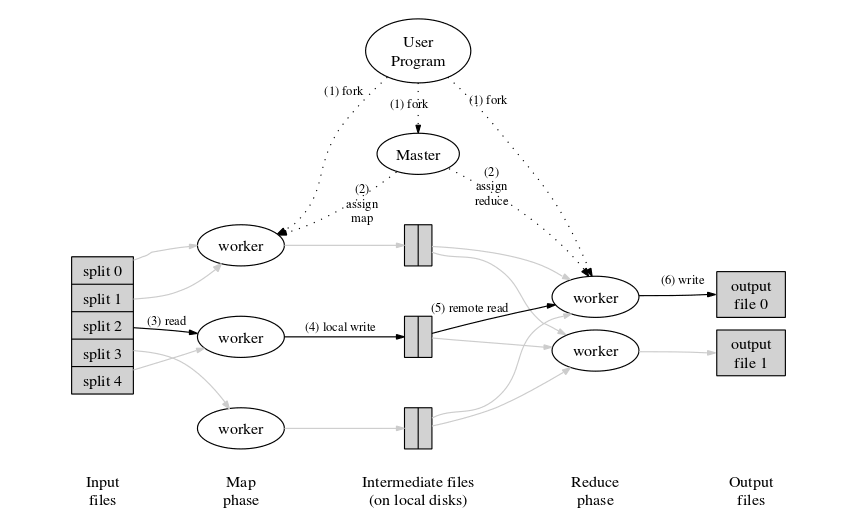
\includegraphics[width=\linewidth]{map-reduce-overview}
  \caption[MapReduce编程模型]{MapReduce编程模型(摘自Google MapReduce论文\cite{Dean2008})}
  \label{fig:map-reduce-overview}
\end{figure}

MapReduce由Google提出\upcite{Dean2008},最初被设计为用于分布式存储计算机集群,
部署在Google的服务器集群之上,执行大规模网络事务处理任务,如网页检索等,表现出很好的性能。
Apache基金会的Hadoop是分布式存储计算机集群上最著名的MapReduce实现。
L\"ammel使用Haskell语言给MapReduce的语义做了精确描述\upcite{Lammel2008}。

Ranger等\upcite{Ranger2007}在共享内存处理器上实现了MapReduce,名为Phoenix,
为MapReduce模型的处理过程提供了更多可配置选项。Phoenix-2是\upcite{Yoo2009}是Phoenix
的改进实现。

MapReduce也被移植到GPU上。香港科技大学的Bingsheng He等在Nvidia GPU上实现了
Mars\upcite{He2008},这是第一个运行在GPU上的Mapreduce系统。由于当时的GPU不支持
动态内存分配,Mars设计了一轮额外的\texttt{map\_count}阶段与一轮额外的\texttt{reduce\_count}
阶段,这带来了一定的附加开销。

MapCG\upcite{Hong2010}是MapReduce系统在GPU上另一版实现。MapCG的贡献是,
统一了MapReduce在CPU端与GPU端的接口设计,并在GPU上实现了一个轻量的动态内存分配器,
从而避免了Mars插入额外处理的开销。

Fang\upcite{Fang2011}增强了了Mars实现,使Mars可以运行在更多并行硬件之上,包括多核CPU、
Nvidia GPU、AMD GPU等,在开发CPU与GPU同时执行计算任务方面进行了一些尝试,
但并未取得理想效果。

Feng\upcite{Ji2011}与Chen\upcite{Chen2012}就GPU片上共享存储器的利用对MapReduce在GPU上
的实现分别提出了不同的优化措施。

Stuart设计了运行在GPU集群上的MapReduce系统GPMR\upcite{Stuart2011}。
出于性能考虑,GPMR向用户暴露了更多硬件细节。GPMR在\texttt{map}阶段
采用了了流水化的执行方式以重叠计算任务与设备间通信。

%% \section{GPU并行编程技术}\label{sec:gpu-parallel-prog}
%% 本节介绍当前使用最广泛的在GPU上进行通用编程的软件技术。

%% \subsection{CUDA}
%% CUDA架构是Nvidia公司针对自己的GPU提出的并行编程框架。
%% 它的提出对GPU通用编程技术产生了巨大的推动力。

%% CUDA为程序员提供了一个完整的GPU编程框架,将GPU的硬件结构
%% 清晰地展现出来。用户使用CUDA C编写在GPU上执行的程序,通常
%% 称为Kernel。CUDA C是一种对C语言的简单扩展,
%% 增加了若干关键字指定程序的执行位置(CPU还是GPU)、变量
%% 的存储位置(全局存储还是贡献存储),
%% 提供了一些内置变量一边获得某些运行时信息。

%% CUDA采用STMD编程模型,这是一种类似与SPMD的编程模型,
%% 一个Kernel程序被一组线程执行,执行路径一般和线程在组中所处的位置相关。
%% 线程按照层次化组织,grid

%% \subsection{OpenCL}

%% \subsection{OpenACC \& OpenHMPP}

\chapter{Rat语法设计}\label{chap:frontend}
Rat语言语法设计的首要目标是为编程者提供易用的并行语言要素,可以简洁优雅地
描述并行问题。

Rat是一种函数式并行程序语言,它具备函数式语言的一般特性:高阶函数、恒值对象、
纯函数特性等,抽象表达能力,问题描述简洁优雅;它面向科学与工程计算领域,强化
数值计算,弱化符号计算,支持定长整数与浮点数类型,这不同于一般函数式语言;
它是一种静态强类型语言,在编译期执行类型检查,运行时安全性较强,无动态类型
检测开销;它提供了一组向量原语,可用来描述一大类数据并行操作;它被设计为一门
辅助性程序语言,为与C语言交互设计了有简单易用的接口,编程者一般只使用Rat语言编写
程序中的数据并行部分。

本章的内容结构如下:
%% 第\ref{sec:rat-overview}节对Rat语言做简单综述,
第\ref{sec:type-system}节介绍Rat的类型系统,
第\ref{sec:vector-primitives}节介绍Rat的核心并行语言要素---向量原语,
第\ref{sec:functional-characters}节对Rat语言采用的函数式语言特性进行说明,
并说明选取函数式语言设计的优势,
第\ref{sec:c-interface}节介绍Rat程序与C语言的交互界面,
第\ref{sec:n-body}节给出一个完整并行程序示例---n-body问题用以说明Rat语言的易用性。

%% \section{Rat语言综述}\label{sec:rat-overview}

\section{类型系统}\label{sec:type-system}
\subsection{Rat支持的数据类型}
在一般的程序语言中,数据与操作(函数、过程)是不同的概念,
数据就是存储在计算机当中的“数”,而操作表示施加在数据上的程序行为。
在函数式程序语言中,数据与函数的界限是模糊的,二者只不过具有不同的类型而已。
Rat是函数式语言,采用类似于Haskell的类型系统,支持数据类型与函数类型。
为了便于理解,在本节中,我们依旧区分“数据”与“函数”,下面分别予以介绍。

\subsubsection{数据类型}
Rat将数据分为两类:标量数据类型(scalar type)与向量类型(vector type)。
其中向量类型是同质(homogeneous)标量类型的一维集合。表\ref{tbl:rat-datatype}列举了
Rat的内建数据类型。

标量类型包括内建数据类型(builtin type),元组类型(tuple)。内建数据类型是计算机能够表示的基本
数据类型,包括定长整数与定长浮点数。而且,由于Rat语言面向科学计算领域,
强化数值计算能力,弱化符号计算能力。所以,Rat内建的基本数据
数据类型只包括定长整数类型与定长浮点数类型。

元组类型也称结构类型(struct),允许不同类型的元素组合得到,Rat的元组类型允许嵌套定义。

向量类型是一个同质数据集合,它包含的数据个体相同的类型,并且必须是标量类型。在Rat语言中
使用方括号表示向量类型,如\texttt{[Int32]}表示一个32位整数向量类型。
向量是一维数据集合,Rat在语法层面不支持高维数组,但通过定义元组及相应的函数可以轻松构建高维
数组程序库。向量类型是Rat语言提供数据并行能力的数据基础,这一点将在第\ref{subsub:vector-primitives}
中详细说明。

\begin{table}[htbp]
  \centering
  \caption{Rat数据类型}
  \label{tbl:rat-datatype}
  \begin{tabularx}{\linewidth}{|l|l|l|X|}
    \hline
    \multirow{11}*{标量类型} &
    \multirow{10}*{内建数据类型} & Int8 & 8 bit 有符号整数\\
    \cline{3-4}
    & & UInt8 & 8 bit 有符号整数\\
    \cline{3-4}
    & & Int16 & 16 bit 有符号整数\\
    \cline{3-4}
    & & UInt16 & 16 bit 有符号整数\\
    \cline{3-4}
    & & Int32 & 32 bit 有符号整数\\
    \cline{3-4}
    & & UInt32 & 32 bit 有符号整数\\
    \cline{3-4}
    & & Int64 & 64 bit 有符号整数\\
    \cline{3-4}
    & & UInt64 & 64 bit 有符号整数\\
    \cline{3-4}
    & & Float & 32 bit 单精度浮点数\\
    \cline{3-4}
    & & Double & 64 bit 双精度浮点数\\
    \cline{2-4}
    & 元组类型 & (a, b, ...) & 其中a, b是任何类型(非函数类型)\\
    \hline
    \multicolumn{2}{|l|}{向量类型} & [a] & 元素类型为a的向量类型,a为标量类型\\
    \hline
  \end{tabularx}
\end{table}

\subsubsection{函数类型}
Rat是函数式语言,支持高阶函数等函数式语言特性,这将在第\ref{sec:functional-characters}节
详细介绍。这里只说明Rat函数的类型表示方法。

一个函数的类型由其输入参数的类型与输出结果的类型唯一决定,下面举例说明。

\begin{quotation}
  \kai{
    \texttt{dot}函数求两个单精度浮点向量的内积,它的类型声明如下:\\
    \centering\texttt{dot :: [Float] -> [Float] -> Float}\\
    其中,最后一个箭头右侧
    的类型表示dot函数返回一个\texttt{Float}类型的结果,前面两个\texttt{[Float]}表示\texttt{dot}
    函数以两个\texttt{[Float]}类型的单精度浮点向量作为输入参数。至于为什么\texttt{dot}的类型
    声明中有多于一个箭头,这与柯里化相关,这部分内容请参见第\ref{sec:functional-characters}节。
  }
\end{quotation}

\subsection{静态强类型}
Rat是一种静态强类型语言,在编译期执行严格的类型检查,保证数据类型与施加在数据上的函数类型
严格匹配。采用静态强类型的类型系统可以获得两方面优势:
\begin{itemize}
  \item 安全性:强类型检查可以保证类型安全,从而避免一大类运行时错误。
    强类型检查的内容包括,所有函数(数据)的类型皆在编译期确定;
    任何函数(数据)的类型在生命周期中保持不变;
    保证所有数据操作的有效性;不允许类型转换操作。
    Rat语言采用的类型系统类似于Haskell,而使用过Haskell
    的编程者都会有体会,那就是程序只要通过了编译,基本不会发生运行时错误。
  \item 高效率:静态类型在运行时没有类型识别与检测的额外开销,可以提高执行效率,这与Rat面向
    科学工程计算的设计初衷相符合。
\end{itemize}

\subsection{多态}
采用静态强类型系统的一个缺点就是编程灵活性受到了限制,特定类型的函数只能作用于
特定类型的数据。但本文认为,为了安全与性能承受灵活性方面的这一点代价是值得的。

为了提高编程灵活性,Rat为函数多态提供了支持。多态是指
同一种逻辑操作可以施加在多种不同类型的数据之上,如加法运算既适用于整型数,也
适用于浮点数。

多态技术可以为编程提供极大的灵活性。如果没有多态的支持,同样的加法运算就需要为不同类型
分别定义,而多态允许“一次定义,多个实例”。多态技术的典型代表是C++ template,
它定义函数或对象模板,以类型作为模板参数,使用时再根据不同的需求进行实例化。
下面的代码片段展示了使用C++ template定义的多态加法函数。
\begin{lstlisting}[language=C++]
template <typename T>
T add (T a, T b) {
  return a+b;
}
\end{lstlisting}

Rat支持多态的方式与Haskell相同,通过引入类型类(type class)的概念实现多态。
一个类型类是一组类型的集合,这些类型具有某些相同的性质,支持某些相同的操作。
如Num类型类是“数”类型的集合,他们都支持加减法运算。为了使用多态,
编程者先定义一个类型类,声明属于该类型类的类型应该支持的方法,
然后将某个类型实例化为该类型类的成员,下面的Rat代码说明了使用多态的方法。
\begin{lstlisting}[language=Haskell]
class Num a where
  + :: a -> a -> a
  - :: a -> a -> a

instance Num Int32 where
  + a b = addInt32 a b
  - a b = substractInt32 a b
\end{lstlisting}

\section{向量原语}\label{sec:vector-primitives}
Rat语言的定位是数据并行语言,采用一种数据并行编程模型。数据并行问
题的特点是,将相同的操作施加到不同的数据上,不同数据操作之间的相关性较
弱,可并行度高。数据并行模型是一种层次较高的并行编程模型,编程者只需要
指出施加在数据上的操作以及该接受该操作的数据集就能实现程序的并行执行,
因此,数据并行问题的描述具有简洁优雅的特点。同时,数据并行问题涵盖了一
大类科学与工程计算问题,应用场景非常广阔。

Rat提供了一组向量原语(Vector Primitive, VP),参见表\ref{tbl:vector-primitives}。
每一个向量原语定义一种施加在一维向量上的并行操作。从表\ref{tbl:vector-primitives}
中可以看出,Rat提供的这一组向量原语集合非常精简,一共只有六个,而仅仅通过组合使用这六种向量原语
就方便地描述一大类数据并行问题。表\ref{tbl:derived-vector-operations}列举了一些在
Rat向量原语基础上可以实现的常见向量操作。

\begin{table}[htb]
  \centering
  \caption{向量原语}
  \label{tbl:vector-primitives}
  \begin{tabularx}{\linewidth}{p{10em}X}
    \toprule[1.5pt]
    \hei{向量原语} & \hei{类型声明} \\
    \midrule[1pt]
    map & (a -> b) -> [a] -> [b]\\
    scan & ScanDirection -> InclusiveMode -> (a -> a -> a) -> [a] -> [a]\\
    slice & Integral i => (i, i) -> [a] -> [a]\\
    gpermute & Integral i => PermuteDirection -> (i -> i) -> [a] -> [a]\\
    gcopy & Boolean b => [b] -> [a] -> [a]\\
    sort & (a -> a -> Ording) -> [a] -> [a]\\
    \bottomrule[1.5pt]
  \end{tabularx}
\end{table}

\begin{table}[htb]
  \centering
  \caption{派生向量操作}
  \label{tbl:derived-vector-operations}
  \begin{tabularx}{\linewidth}{p{10em}X}
    \toprule[1.5pt]
    \hei{向量原语} & \hei{类型声明} \\
    \midrule[1pt]
    fold & (a -> a -> a) -> [a] -> a\\
    permute & Integral i =>(i -> i)-> [a] -> [a]\\
    backpermute & Integral i =>(i -> i)->[a] -> [a]\\
    scale & Integral i => ScaleType -> i -> [a] -> [a]\\
    compact & Boolean b => [b] -> [a] -> [a]\\
    sparse & Boolean b => [b] -> [a] -> [a]\\
    filter & Boolean b => (a -> b) -> [a] -> [a]\\
    reverse & [a] -> [a]\\
    \bottomrule[1.5pt]
  \end{tabularx}
\end{table}

下面分别对各个向量原语进行说明,给出他们的严格语义定义,
图\ref{fig:vp-diagrams}是各向量原语的操作示意图。

\subsection{map}
map原语以一个标量操作与一个向量为输入参数,标量操作的类型与输入向量的类型
严格匹配。map原语对向量中的所有数据个体施加同一操作,然后收集结果
返回一个新的向量。
\begin{definition}
  map原语以一个一元函数$f$与一个向量$$[a_0, a_1, \cdots, a_{n-1}]$$作为输入参数,
  返回一个向量$$[f(a_0), f(a_1), \cdots, f(a_{n-1})]$$作为结果。
\end{definition}

图\ref{fig:map-diagram}给出map原语的操作说明。
\begin{figure}[h]
  \centering
  \includegraphics[height=4cm]{map}
  \caption{map原语操作示意图}
  \label{fig:map-diagram}
\end{figure}

\subsection{slice}
slice原语对一个向量执行截断操作,他以一对整数\texttt{(i, j)}作为向量
截断的起点与重点,截取输入向量的一段作为输出向量。\texttt{(i, j)}表示
一个前闭后开区间,即$[i, j)$。图\ref{fig:slice-diagram}给出了slice原语的操作说明。
\begin{definition}
  slice原语以一对整数$(i, j)$与一个向量$$[a_0, a_1, \cdots, a_{n-1}]$$作为输入参数,
  其中$0\le{}i<j\le{}n-1$,返回一个向量$$[a_{i}, \cdots, a_{j-1}]$$作为结果。
\end{definition}

图\ref{fig:slice-diagram}给出slice原语的操作说明。
\begin{figure}[h]
  \centering
  \includegraphics[height=4cm]{slice}
  \caption{slice原语操作示意图}
  \label{fig:slice-diagram}
\end{figure}

\subsection{scan}
scan原语又称为prefix-sum,它使用一个满足结合律的二元函数对输入向量做部分和累加操作。scan原语提供两个配置选项:
累加方向\texttt{ScanDirection}与头部元素包含模式\texttt{InclusiveMode}。
\begin{definition}
  scan原语以一个满足结合律以$I$为幺元的二元函数$\oplus$与一个向量$$[a_0, a_1, \cdots, a_{n-1}]$$作为输入,
  根据两个配置参数  $ScanDirection, InclusiveMode$的取值返回一个部分和向量作为结果。
  不同配置参数下的返回结果如下:\\
  $[a_0, (a_0\oplus{}a_1), \cdots, (a_0\oplus{}\cdots\oplus{}a_{n-1})]$\hfill{}Inclusive, Forward\\
  $[(a_0\oplus\cdots\oplus{}a_{n-1}), \cdots, (a_{n-2}\oplus{}a_{n-1}), a_{n-1}]$\hfill{}Inclusive, Backward\\
  $[I, a_0, (a_0\oplus{}a_1), \cdots, (a_0\oplus{}\cdots\oplus{}a_{n-2})]$\hfill{}Exclusive, Forward\\
  $[(a_1\oplus\cdots\oplus{}a_{n-1}), \cdots, (a_{n-2}\oplus{}a_{n-1}), a_{n-1}, I]$\hfill{}Exclusive, Backward\\
  %% \begin{tabular}{|l|l|l|}
  %%   \hline
  %%   %% \backslashbox{ScanDirection}{InclusiveMode}
  %%   & Inclusive & Exclusive\\
  %%   \hline
  %%   Forward & $[a_0, (a_0\oplus{}a_1), \cdots, (a_0\oplus{}\cdots\oplus{}a_{n-1})]$ &
  %%   $[I, a_0, (a_0\oplus{}a_1), \cdots, (a_0\oplus{}\cdots\oplus{}a_{n-2})]$ \\
  %%   \hline
  %%   Backward & $[(a_0\oplus\cdots\oplus{}a_{n-1}), \cdots, (a_{n-2}\oplus{}a_{n-1}), a_{n-1}]$ &
  %%   $[(a_1\oplus\cdots\oplus{}a_{n-1}), \cdots, (a_{n-2}\oplus{}a_{n-1}), a_{n-1}, I]$ \\
  %%   \hline
  %% \end{tabular}
\end{definition}

图\ref{fig:scan-diagram}给出scan原语的操作说明。
\begin{figure}[h]
  \centering
  \subfloat[Inclusive, Forward]{
    \includegraphics[height=4cm]{scan-if}\hspace{2em}
  }
  \subfloat[Exclusive, Forward]{
    \includegraphics[height=4cm]{scan-ef}\hspace{2em}
  }
  \\
  \subfloat[Inclusive, Backward]{
    \includegraphics[height=4cm]{scan-ib}\hspace{2em}
  }
  \subfloat[Exclusive, Backward]{
    \includegraphics[height=4cm]{scan-eb}\hspace{2em}
  }
  \caption{scan原语操作示意图}
  \label{fig:scan-diagram}
\end{figure}

\subsection{gpermute}
gpermute对一个向量执行通用乱序操作,它以一个索引计算函数与一个向量为输入,接受一个配置参数PermuteDirection。
\begin{definition}
  gpermute原语以一个索引计算函数$g$与一个向量$$[a_0, a_1, \cdots, a_{n-1}]$$作为输入,
  根据配置参数  $PermuteDirection$的取值返回一个重排序的向量作为结果。
  不同配置参数下的返回结果如下:\\
  $[a_{g^{-1}(0)}, a_{g^{-1}(1)}, \cdots, a_{g^{-1}_{n-1}}]$\hfill{}Forward\\
  $[a_{g(0)}, a_{g(1)}, \cdots, a_{g_{n-1}}]$\hfill{}Backward\\  
\end{definition}

图\ref{fig:gpermute-diagram}给出gpermute原语的操作说明。
\begin{figure}[h]
  \centering
  \subfloat[Forward]{
    \includegraphics[height=4cm]{gpermute-f}
  }
  \\
  \subfloat[Backward]{
    \includegraphics[height=4cm]{gpermute-b}
  }
  \caption{gpermute原语操作示意图}
  \label{fig:gpermute-diagram}
\end{figure}

\subsection{gcopy}
gcopy原语以一个标志向量与一个数据向量为输入,根据标志向量中数据的真值确定是否对数据向量
中相应位置的元素执行拷贝,将所有拷贝的数据收集起来得到结果。
\begin{definition}
  gcopy原语以一个标志向量$$[b_0, b_1, \cdots, b_{n-1}]$$与一个数据向量$$[a_0, a_1, \cdots, a_{n-1}]$$作为输入,
  返回一个向量$$[a_{n_1}, a_{n_2}, \cdots, a_{n_k}]$$作为结果,其中$0\le{}n_1<n_2<\cdots{}<n_k\le{}n-1$且
  $b_{n_i}=true, i=1,2,\cdots,k$。
\end{definition}

图\ref{fig:gcopy-diagram}给出gcopy原语的操作说明。
\begin{figure}[h]
  \centering
  \includegraphics[height=4cm]{gcopy}
  \caption{gcopy原语操作示意图}
  \label{fig:gcopy-diagram}
\end{figure}

\subsection{sort}
sort原语以一个比较函数与一个向量作为输入,返回一个结果向量,其中的元素皆来自输入向量,
但任何一个元素都比位于它后面的元素“小”。
\begin{definition}
  sort原语以一个二元比较函数$\prec$与一个向量$$[a_0, a_1, \cdots, a_{n-1}]$$作为输入,
  返回一个结果向量$$[a_{n_1}, a_{n_2}, \cdots, a_{n_n}]$$,该向量是输入向量的一个重排,
  并且对于任意$n_i\prec{}n_j$都有$a{n_i}\prec{}a{n_j}$。
\end{definition}

图\ref{fig:sort-diagram}给出sort原语的操作说明。
\begin{figure}[h]
  \centering
  \includegraphics[height=4cm]{sort}
  \caption{sort原语操作示意图}
  \label{fig:sort-diagram}
\end{figure}

%% 下面使用一个简单例子说明数据并行问题的特点。
%% \begin{quotation}
%%   求解两个向量$u, v$的内积FIXME:equation and font
%%   $$d=u\cdot{}v=\sum_{k=1}^nu_kv_k$$
%% \end{quotation}

\section{函数式语言特性}\label{sec:functional-characters}
Rat采用了函数式语言设计,具备函数式程序语言的一般特点。在本章的后续各节中
将分别介绍Rat采用的函数式语言特性,并在最后进行总结,说明采用函数式设计带来的优势。

\subsection{函数“一等公民”}
函数式程序语言采用的计算模型是$\lambda$演算($\lambda$ Calculus)理论FIXME:citehere,是一种在功能上等价于
图灵机的计算模型FIXME:citehere。Rat是一种强类型语言,
它的理论基础是$\lambda$演算的一个扩展---类型$\lambda$演算(Typed $\lambda$ Calculus)。
在$\lambda$演算的形式化系统中,所有公式都可以看作函数,也就是说,常量被看作0元函数。
命令式语言区分“函数”与“数据”的界限在函数式语言中并不存在,函数与数据是等价的,
函数式语言中函数是一等公民,下面给出其定义:

\begin{definition}
  当程序语言中的函数具备下列性质时,称函数为该语言的“一等公民”(first-class citizen)FIXME:citehere:
  \begin{compactitem}
    \item 函数可以作为参数传递给其他函数,即支持高阶函数;
    \item 函数可以作为其他函数的返回值;
    \item 允许匿名函数
  \end{compactitem}
\end{definition}


\subsection{纯函数特性}
纯函数特性(pure functional)也称为无副作用(side-effect free)。有无副作用
描述的是程序语言中“函数”的一种性质,副作用是指,函数除了在返回某个值以外,
还改变了某些全局状态,或与程序外部的世界发生了交互。副作用,是程序语言中“函数”与数学
中“函数”的主要区别,数学函数单纯地使用输入参数计算一个返回值,而程序函数除了
计算返回值以外,还可能执行IO操作、引起异常行为等。一般来说,副作用对于程序运行
是必要的,甚至有些程序函数定义的目的就是为引起某些副作用大发生,如IO函数。

而某些程序函数,如数学函数,在执行计算的同时不引起任何副作用。我们称这类函数
为纯函数,其定义如下:
\begin{definition}
纯函数(pure function),指不引起任何副作用,
计算结果只与输入参数相关,无论何时,只要给定相同输入,就保证返回相同结果的程序函数。
\end{definition}

Rat语言面向科学工程计算设计,它关注的核心任务是数学计算,而数学计算中
使用的函数恰恰满足纯函数的特征。采用纯函数设计,不仅可以简化程序语言的
语义分析,更为程序的自动并行化提供了巨大的便利,
这将在第\ref{subsec:functional-advantages}节详细说明。

\subsection{柯里化}
柯里化(curried)也是程序函数的一种性质,它实质上是允许程序函数的形式参数
部分实例化,得到的结果仍是一个函数,这个函数的形式参数就是原函数未被实例化
的形式参数。下面仍以求解向量内积的例子说明。
\begin{quotation}
  \kai{
    \texttt{dot}函数求两个单精度浮点向量的内积,它的类型声明如下:\\
    \texttt{dot :: [Float] -> [Float] -> Float}\\
    \texttt{dot}函数有两个形式参数,当按照如下方式调用\texttt{dot}函数时,
    将可以得到两个向量\texttt{u},\texttt{v}的内积:\\
    \texttt{s = dot u v}\\
    但如果只对一个形式参数实例化,即按照如下方式调用,
    将得到一个一元函数\texttt{dotWithU},
    它有只有一个形式参数,当对这个形式参数实例化的时候,求解该实参与向量
    \texttt{u}的内积:\\
    \texttt{dotWithU = dot u}\\
    \texttt{s = dotWithU v}
  }
\end{quotation}

柯里化也可以从另一个视角理解,将所有函数都看作一元函数,一个n元函数可以看作
一个返回值为n-1元函数的一元函数。即,在多元函数的类型声明中,箭头\texttt{->}
是右结合的。这样,\texttt{dot}函数的类型声明可以看作:\\
\texttt{dot:: [Float] -> ([Float] -> [Float])}

\subsection{恒值对象}\label{subsec:immutable-object}
恒值对象也是函数式语言的重要特点。需要说明的是,这里的“对象”(object)
不同与面向对象程序语言中的对象,而是函数式语言中唯一的实体类型---函数,
之所以采用“恒值对象”而非“恒值函数”,是因为将“函数”与“赋值”联系起来
不够自然。FIXME:可以介绍传值语义以及命令式函数式混合体设计。

\begin{definition}
  恒值对象,指对象只在其定义的时候被确定其值,在其后的生命周期中不允许再次赋值,
  对象的值在整个生命周期中保持不变。
\end{definition}

Rat语言中的函数(函数与数据的总称)都是恒值对象,所以,严格来讲,Rat不支持
“变量”的概念。

恒值特性是与纯函数特性协调的,因为在现行的冯$\cdot$诺依曼计算机上,对象赋值
就代表内存区域的改写,这必然引起副作用的发生。

\subsection{函数式语言设计的优势}\label{subsec:functional-advantages}
前面介绍了Rat语言采用的若干函数式设计,下面说明为什么要采用函数式语言设计,
上述的函数式语言特性能带来什么优势。

\subsubsection{抽象层次高}
高阶函数与柯里化特性为编程提供了极大灵活性,编程者可以灵活地操作函数,
使用已有的函数构建新函数;

恒值对象将编程者从内存管理的工作中解脱出来,只需集中注意力在解决问题的逻辑
之上,内存等硬件资源的有效利用由编译期与运行时系统负责。

此外,高阶函数的使用大大增强了程序的表达能力,使得复杂的问题可以用
非常简洁优雅的代码就可以描述,且程序代码逻辑性强,可读性强。

\subsubsection{语义简单精确}
纯函数特性与恒值对象使得程序的语义更加简单精确,大大降低了语义分析的难度,
这样就使得编译器更容易掌握程序行为,同时也使得程序的高层优化更容易进行。

\subsubsection{为程序并行化提供支持}
函数式语言的理论基础是$\lambda$演算,程序的运行实质就是$lambda$演算理论中
表达式求值的过程。表达式求值的基本形式是函数应用(function application),即
通常所说的函数调用:将函数形式参数实例化,计算返回值。一个复杂表达式可能由
多个子表达式构成,各个子表达式的求值先于整个表达式的求值。

如果一个表达式中应用的函数都是纯函数,那么由$\lambda$演算理论中的
Church-Rosser定理(也称为菱形性质)FIXME:citehere可以得到下面的定理:
\begin{theorem}
  一个表达式的求值结果与子表达式的求值顺序无关。
\end{theorem}

上述定理表明,纯函数特性为程序自动并行化提供了有力支持,一个复杂表达式的
各个子表达式可以并行求值,同时保证得到正确的最终结果!

\begin{quotation}
  \kai{
    考虑下面的表达式求值问题:\\
    \texttt{dot (map f u) (scan g v)}\\
    表达式求值过程可以以一棵求值树表示,树中每一个非叶结点表示一个函数应用,
    叶结点表示函数或者数据,求值过程自下向上,最终得到根结点的值即为整个表达式的
    求值结果。上述表达式的求值树如图\ref{fig:expression-tree},其中分别以
    \texttt{t1}与\texttt{t2}为根的两棵子树代表的子表达式可以并行求值。
  }
\end{quotation}
\begin{figure}
  \centering
  \includegraphics[height=5cm]{expression-tree}
  \caption{表达式求值树}
  \label{fig:expression-tree}
\end{figure}

\section{C语言接口}\label{sec:c-interface}
正如第\ref{subsec:functional-advantages}节所说,纯函数特性是一种非常优良
的语言特性,但副作用在程序设计中也是必不可少的,因为程序要解决问题,不光
要做计算的工作,还必须与外部世界发生交互,如从外部存储器读取输入,向外部写入
计算结果等等。

如何在保留纯函数特性优势的前提下,允许副作用的发生呢?不同函数式语言有不同做法,
Lisp系语言与ML系语言不是纯函数式的,允许副作用发生,Haskell采用一种MonadFIXME:citehere
技术将程序的纯函数部分与副作用部分严格隔离开来,以便在纯函数部分仍旧能够利用
纯函数特性带来的优良性质。

Rat采用了一种不同的策略。Rat主要的设计目标是降低并行程序设计
的难度,提供易用性强的并行编程工具,由于它是一种数据并行语言,面向
科学与工程计算,所以程序的并行部分集中在计算过程,这部分程序是无副作用的。
所以,Rat被设计用来与C语言协同工作,程序的副作用部分,一般也是串行部分(如IO操作等)
使用C语言编写,计算的部分,一般也是并行性所在的部分,使用Rat语言编写。
Rat提供简单易用的C语言交互接口,允许C语言调用Rat程序。实际上,Rat编译器
就是一个源到源(source-to-source)编译器,它将Rat程序翻译成C函数供C程序调用。

Rat的C语言交互接口非常简单,仅包含一个export语句。export语句的形式语法参见附录FIXME:refhere。
通过export语句,Rat编译器将使用Rat语言定义的函数提供给C语言使用,C语言可以调用Rat函数完成
计算任务。

FIXME:有关数据类型映射的表格可以添加
%% Rat的C语言交互接口包括两个语法:import语句与export语句。
%% \begin{itemize}
%%   \item import语法形式如下:\\
%%     \texttt{import \textsl{<identifier> :: <type>}}\\
%%     该语法从外部引入一块数据,以\texttt{\textsl{identifier}}作为引用名称,
%%     其类型为\texttt{\textsl{type}}
%% \end{itemize}

\section{Rat程序实例---n-body问题}\label{sec:n-body}
本节使用Rat语言解决一个实际问题---n-body问题,以此展示Rat语言强大的抽象能力与
表达能力,同时展示Rat语言隐藏并行细节的能力。FIXME:font
\begin{quotation}
  \kai{
    n-body问题是一个经典数据并行问题。问题描述如下:

    在一个二维空间内存在$n$个粒子$[cell_1, cell_2, \cdots, cell_n]$,
    粒子具有质量$m$,位置$(P^x,P^y)$,速度$(V^x, V^y)$三种属性,
    粒子相互之间存在引力,粒子$i$与粒子$j$相互之间引力大小与他们的质量成正比,
    与距离平方成反比,即$F=G\frac{m_im_j}{D}$,
    其中$G$为引力常数,
    $D=(p^x_i-p^x_j)^2+(P^y_i-P^y_j)^2$为两个粒子间的距离。
    给定$n$个粒子的的质量$[m_1, m_2, \cdots, m_n]$,
    初始位置$[(P^x_1, P^y_1), (P^x_2, P^y_2), \cdots, (P^x_n, P^y_n)]$,
    与初始速度$[(V^x_1, V^y_1), (V^x_2, V^y_2), \cdots, (V^x_n, V^y_n)]$,
    以$t$为时间步长,求解第$n$个粒子从$0$时刻起每个时间步长之后的位置。
  }
\end{quotation}

n-body问题的Rat实现如下,下面对代码中的关键部分予以说明。
\begin{compactitem}
  \item 第1行的export语句表示,将\texttt{solveNBodyOneStep}函数
    输出给C程序调用,生成的C函数类型与solveNBodyOneStep在Rat语言中的类型相对应。
  \item 第3-10行定义需要使用的数据类型,这些数据类型都有对应的C语言结构类型。
    其中位置\texttt{Position}与速度\texttt{Velocity}都由一对浮点数组成,
    质量\texttt{Mass}是一个浮点数,例子\texttt{Cell}由它的三种属性构成。
  \item 第12-13行定义了引力常数\texttt{g}
  \item 第15-34行定义了完成计算功能的函数\texttt{solveNBodyOneStep},
    该函数以时间步长\texttt{t}与一组粒子\texttt{cells}为输入参数,计算\texttt{t}
    时间后粒子状态。
    \begin{compactitem}
      \item 第19-27行定义了一些辅助函数与中间变量,
        \texttt{positions}包含所有粒子的位置,\texttt{velocities}包含了所有粒子的初始速度,
        \texttt{calcDistanceSqure}计算两个粒子距离的平方和,
        \texttt{calcSingleAcc}计算单个粒子对给定粒子造成的加速度。
      \item 第28-29行定义\texttt{calcAccelerate}计算所有粒子对给定粒子造成的加速度和,
        使用了\texttt{fold}方法。
      \item 第30行定义的\texttt{accelerates}包含所有粒子在当前状态下受力产生的加速度。
      \item 第31-34行计算$t$时间后粒子的速度\texttt{newVelocities}与位置\texttt{newPositions},
        使用了\texttt{zipWith}方法。
      \item 第17行根据计算得到的$t$时间后的粒子位置与速度生成新的粒子状态,
        使用了\texttt{zipWith3}方法。
    \end{compactitem}
\end{compactitem}

\lstinputlisting[language=Haskell]{listings/nbody.hs}

14527321327

\chapter{Rat编译实现技术}\label{chap:compiler}
第\ref{chap:frontend}章介绍了Rat语言的语法设计,简洁优雅的语法为编程者提供了
良好的编程界面,解决了并行编程工具的易用性问题。那么另一方面,
高效性要依靠语言的编译实现技术解决。

本章将详细说明Rat语言编译实现的关键技术,包括中间语言Core的设计,
流驱动并行计算模型的使用与流探测技术,两种流优化算法以及最终的代码生成方案。
本章内容结构安排如下:
第\ref{sec:compiler-overview}节介绍Rat语言编译实现的总体方案,总览Rat程序的编译流程。
第\ref{sec:core-language}节给出了Core语言的设计,Core语言为Rat提供了数值计算能力与
数据并行能力,它提供的向量原语是可以在多种并行硬件上高效实现的。
第\ref{sec:stream-detection}节说明流探测技术,该算法是Rat编译实现中最为关键的算法,是并行任务生成的基础。
%% 第\ref{sec:np-decomposition}节说明嵌套并行的分解技术,它的功能是将嵌套并行操作分解
%% 为一维并行操作序列。
第\ref{sec:stream-optimization}节介绍若干高层优化技术,这些高层优化技术
施加在向量流上。
第\ref{sec:code-generation}节介绍如何从程序的向量流图生成C代码。

\section{编译实现总体方案}\label{sec:compiler-overview}
第\ref{sec:c-interface}节已经提到,Rat编译器是一个源到源编译期,
最终产生C语言代码,将Rat函数转换成合适类型的C语言函数供C程序调用。
图\ref{fig:frontend}给出了从Rat代码到C代码的翻译流程,步骤如下:
\begin{enumerate}
  \item Rat代码经过词法分析器与语法分析器,形成L1语法树。
    L1语法树是Rat代码的直接表示,它包含的结点类型参见表\ref{tbl:l1-ast}。
  \item L1语法树经过L1变换得到L2语法树。L2语法树结构更加简单,包含的结点类型
    更少,参见表\ref{tbl:l2-ast}。
  \item L2语法树经过L2变换得到Core语法树。Core语法树是Core语言的树状表示,
    Core语法树的结点类型同L2语法树。
  \item Core语法树经过流探测算法转化成向量流图表示。
  \item 在向量流图层面实施若干高层优化技术。
  \item 程序从向量流图形式最后被翻译成C语言程序,该C程序是对Rat运行时系统的API调用,
    运行时系统将在下一章介绍。
\end{enumerate}
\begin{figure}[tbh]
  \centering
  \includegraphics[width=\linewidth]{frontend}
  \caption{Rat编译流程}
  \label{fig:frontend}
\end{figure}
\begin{table}[tbh]
  \centering
  \caption{L1语法树结点类型}\label{tbl:l1-ast}
  \begin{tabularx}{\linewidth}{ZZ}
      \toprule[1.5pt]
      {\hei 结点类型} & {\hei 描述} \\
      \midrule[1pt]
      type-define & 类型定义\\
      object-decl & 对象声明\\
      object-def & 对象定义\\
      object-ref & 对象引用\\
      literal & 字面量\\
      function-app & 函数应用\\
      lambda-exp & 函数定义\\
      conditional & 条件表达式\\
      vector-comprehension & 向量推导\\
      vector-ele-ref & 向量元素引用\\
      vector-slice-ref & 向量片段引用\\
      local-binding & 局部定义\\
      \bottomrule[1.5pt]
    \end{tabularx}
\end{table}
\begin{table}[tbh]
  \centering
  \caption{L2语法树与Core语法树结点类型}\label{tbl:l2-ast}
  \begin{tabularx}{\linewidth}{ZZ}
      \toprule[1.5pt]
      {\hei 结点类型} & {\hei 描述} \\
      \midrule[1pt]
      object-ref & 对象引用\\
      literal & 字面量\\
      function-app & 函数应用\\
      lambda-exp & 函数定义\\
      conditional & 条件表达式\\
      \bottomrule[1.5pt]
    \end{tabularx}
\end{table}

\section{Core语言}\label{sec:core-language}
Core语言是一种结构简单的语言,容易分析,并且支持若干高层优化技术。

Core语言的指令集庞大,但结构相对简单,只包含三类指令:向量原语、标量原语和
辅助指令。
其中,标量原语提供了数值计算能力,
向量原语提供了并行计算能力。两类指令构成了一种简单而强大
的计算模型,非常适合表达实际的数据并行问题。
辅助指令提供一些附加功能。

\subsection{向量原语}\label{subsec:vector-primitives}
Core语言提供了一组非常精简的并行操作原语,它包括了一些最为基本的向量操作,这些操作
最为重要的特点是非常适合并行实现。
事实上,正是这组原语为Rat提供了数据并行能力。
表\ref{tbl:vector-primitives}列出了所有向量原语。
\begin{table}[htb]
  \centering
  \caption{向量原语}
  \label{tbl:vector-primitives}
  \begin{tabularx}{\linewidth}{p{10em}X}
    \toprule[1.5pt]
    \hei{向量原语} & \hei{功能说明} \\
    \midrule[1pt]
    \texttt{map} & 给定一元操作,对一个向量中所有元素施加同一操作\\
    \texttt{scan} & 给定满足结合律的二元操作,求一个向量中元素的部分和\\
    \texttt{gpermute} & 对向量中的元素重排\\
    \texttt{gcopy} & 对向量中的元素采取特定步长复制\\
    \texttt{shrink} & 对给定向量采取紧缩复制\\
    \texttt{sort} & 给定排序函数,对向量中的元素进行排序\\
    \texttt{random} & 产生随机向量\\
    \texttt{generate} & 根据位置产生向量元素\\
    \texttt{zip} & 将多个向量中的元素逐位置组成元组\\
    \bottomrule[1.5pt]
  \end{tabularx}
\end{table}

这组原语存在于典型的函数式语言中,但一般是针对表(List)定义的,其语义也是串行的,
但Core语言的向量原语是并行的,这是一个显著区别。
这组原语的选取受到了MapReduce的启发FIXME:citehere。
使用这组精简的原语集可以构建更多更为复杂的向量操作,
如表\ref{tbl:vector-operations}中列出的\texttt{filter}操作就可以按照如下方式定义:\\
\centerline{\texttt{filter p v = shrink (scan (map p v)) v}}

下面分别给出各向量原语的定义。
\subsubsection{map}
\begin{definition}
  map原语以一个一元函数$f$与一个向量$$[a_0, a_1, \cdots, a_{n-1}]$$作为输入参数,
  返回一个向量$$[f(a_0), f(a_1), \cdots, f(a_{n-1})]$$作为结果。
\end{definition}

图\ref{fig:map-diagram}给出map原语的操作说明。
\begin{figure}[h]
  \centering
  \includegraphics[height=4cm]{map}
  \caption{map原语操作示意图}
  \label{fig:map-diagram}
\end{figure}

\subsubsection{scan}
\begin{definition}
  scan原语以一个满足结合律以$I$为幺元的二元函数$\oplus$与一个向量$$[a_0, a_1, \cdots, a_{n-1}]$$作为输入,
  根据两个配置参数  $ScanDirection, InclusiveMode$的取值返回一个部分和向量作为结果。
  不同配置参数下的返回结果如下:\\
  $[a_0, (a_0\oplus{}a_1), \cdots, (a_0\oplus{}\cdots\oplus{}a_{n-1})]$\hfill{}Inclusive, Forward\\
  $[(a_0\oplus\cdots\oplus{}a_{n-1}), \cdots, (a_{n-2}\oplus{}a_{n-1}), a_{n-1}]$\hfill{}Inclusive, Backward\\
  $[I, a_0, (a_0\oplus{}a_1), \cdots, (a_0\oplus{}\cdots\oplus{}a_{n-2})]$\hfill{}Exclusive, Forward\\
  $[(a_1\oplus\cdots\oplus{}a_{n-1}), \cdots, (a_{n-2}\oplus{}a_{n-1}), a_{n-1}, I]$\hfill{}Exclusive, Backward\\
\end{definition}

图\ref{fig:scan-diagram}给出scan原语的操作说明。
\begin{figure}[h]
  \centering
  \subfloat[Inclusive, Forward]{
    \includegraphics[height=4cm]{scan-if}\hspace{2em}
  }
  \subfloat[Exclusive, Forward]{
    \includegraphics[height=4cm]{scan-ef}\hspace{2em}
  }
  \\
  \subfloat[Inclusive, Backward]{
    \includegraphics[height=4cm]{scan-ib}\hspace{2em}
  }
  \subfloat[Exclusive, Backward]{
    \includegraphics[height=4cm]{scan-eb}\hspace{2em}
  }
  \caption{scan原语操作示意图}
  \label{fig:scan-diagram}
\end{figure}

\subsubsection{gpermute}
\begin{definition}
  gpermute原语以一个索引计算函数$g$与一个向量$$[a_0, a_1, \cdots, a_{n-1}]$$作为输入,
  根据配置参数  $PermuteDirection$的取值返回一个重排序的向量作为结果。
  不同配置参数下的返回结果如下:\\
  $[a_{g^{-1}(0)}, a_{g^{-1}(1)}, \cdots, a_{g^{-1}_{n-1}}]$\hfill{}Forward\\
  $[a_{g(0)}, a_{g(1)}, \cdots, a_{g_{n-1}}]$\hfill{}Backward\\  
\end{definition}

图\ref{fig:gpermute-diagram}给出gpermute原语的操作说明。
\begin{figure}[h]
  \centering
  \subfloat[Forward]{
    \includegraphics[height=4cm]{gpermute-f}
  }
  \\
  \subfloat[Backward]{
    \includegraphics[height=4cm]{gpermute-b}
  }
  \caption{gpermute原语操作示意图}
  \label{fig:gpermute-diagram}
\end{figure}

\subsubsection{gcopy}
\begin{definition}
  gcopy原语以一个整数三元组$(i, j, s)$与一个向量$$[a_0, a_1, \cdots, a_{n-1}]$$作为输入参数,
  其中$0\le{}i<j\le{}n-1$,返回一个向量$$[a_{i}, a_{i+s}, a_{i+2s}, \cdots, a_{j-mod(j-i,s)}]$$作为结果。
\end{definition}

图\ref{fig:gcopy-diagram}给出gcopy原语的操作说明。
\begin{figure}[h]
  \centering
  \includegraphics[height=4cm]{gcopy}
  \caption{gcopy原语操作示意图}
  \label{fig:gcopy-diagram}
\end{figure}

\subsubsection{shrink}
\begin{definition}
  shrink原语以一个位置压缩向量$$[b_0, b_1, \cdots, b_{n-1}]$$与一个数据向量$$[a_0, a_1, \cdots, a_{n-1}]$$作为输入,
  返回一个向量$$[a_{n_1}, a_{n_2}, \cdots, a_{n_k}]$$作为结果。
\end{definition}

图\ref{fig:shrink-diagram}给出shrink原语的操作说明。
\begin{figure}[h]
  \centering
  \includegraphics[height=4cm]{shrink}
  \caption{shrink原语操作示意图}
  \label{fig:shrink-diagram}
\end{figure}

\subsubsection{sort}
\begin{definition}
  sort原语以一个二元比较函数$\prec$与一个向量$$[a_0, a_1, \cdots, a_{n-1}]$$作为输入,
  返回一个结果向量$$[a_{n_1}, a_{n_2}, \cdots, a_{n_n}]$$,该向量是输入向量的一个重排,
  并且对于任意$n_i\prec{}n_j$都有$a{n_i}\prec{}a{n_j}$。
\end{definition}

图\ref{fig:sort-diagram}给出sort原语的操作说明。
\begin{figure}[h]
  \centering
  \includegraphics[height=4cm]{sort}
  \caption{sort原语操作示意图}
  \label{fig:sort-diagram}
\end{figure}

\subsubsection{zip}
图\ref{fig:zip-diagram}给出了zip原语的操作说明。
\begin{definition}
  zip原语以两个等长向量$$[a_0, a_1, \cdots, a_{n-1}]$$ $$[b_0, b_1, \cdots, b_{n-1}]$$作为输入参数,
  返回一个向量$$[(a_0, b_0), (a_1, b_1), \cdots, (a_{n-1}, b_{n-1})]$$作为结果。
\end{definition}

图\ref{fig:zip-diagram}给出zip原语的操作说明。
\begin{figure}[h]
  \centering
  \includegraphics[height=4cm]{zip}
  \caption{zip原语操作示意图}
  \label{fig:zip-diagram}
\end{figure}

\subsection{标量原语}\label{subsec:scalar-primitives}
Core语言提供了数量众多的标量原语,功能为基本的算数逻辑运算与常用数学函数,
这其中囊括了标准C数学库定义的所有数学函数。FIXME:提及附录。

标量原语中有一类需要注意,即某些满足结合律同时存在幺元的操作,
如加法运算、乘法运算、布尔数求与、布尔数求或等。
从代数学的角度上讲,这种运算可以与某种数据类型构成一个幺半群。

对于向量原语\texttt{scan},只有当传递给它的二元操作满足上述性质时,
\texttt{scan}才可以并行执行,所以,只有满足该性质的标量原语可以作为
参数传递给\texttt{scan}。表\ref{tbl:monoid-scalar-primitives}列出了所有满足这种性质
的标量原语。
\begin{table}
  \centering
  \caption{满足结合律的标量原语}
  \label{tbl:monoid-scalar-primitives}
  \begin{tabularx}{\linewidth}{ccXX}
    \toprule[1.5pt]
    \hei{标量原语} & \hei{功能说明} & \hei{幺半群类型} & \hei{幺元}\\
    \midrule[1pt]
    \texttt{+} & 加法 & 所有数值类型 & 0\\
    \texttt{*} & 乘法 & 所有数值类型 & 1\\
    \texttt{and} & 逻辑与 & 整数类型 & \texttt{true}\\
    \texttt{or} & 逻辑或 & 整数类型 & \texttt{false}\\
    \texttt{max} & 最大值 & 所有数值类型 & 该类型可表示的极大值\\
    \texttt{min} & 最小值 & 所有数值类型 & 该类型可表示的极小值\\
    %% \texttt{gcd} & 最大公约数 & 所有整数类型 & \\
    %% \texttt{lcm} & 最大公约数 & 所有整数类型 & \\
    \bottomrule[1.5pt]
  \end{tabularx}
\end{table}

\subsection{辅助指令}
Core语言提供了若干的辅助指令,这部分指令既不属于提供数值计算能力的
标量原语,也不属于提供并行计算能力的向量原语。
表\ref{tbl:assist-instruction}列出了他们的名称及功能。
\begin{table}
  \centering
  \caption{辅助指令}
  \label{tbl:assist-instruction}
  \begin{tabularx}{\linewidth}{p{10em}X}
    \toprule[1.5pt]
    \hei{辅助指令} & \hei{功能说明} \\
    \midrule[1pt]
    \texttt{length} & 返回向量长度\\
    \texttt{vref} & 引用向量某个特定位置的值\\
    %% \texttt{collect} & 将多个同类型数据收集成为一个向量\\
    \texttt{if} & 条件指令,根据条件表达式的值返回不同的值\\
    \texttt{foreach} & 迭代指令,将多个同类型数据收集成为一个向量\\
    \bottomrule[1.5pt]
  \end{tabularx}
\end{table}

需要注意的是,表中的\texttt{if}指令与\texttt{foreach}指令不同于命令式语言
中的相应概念,在命令式语言中二者是一种语法结构,而在Core语言中这两条都是指令,
它们与操作数共同构成表达式,代表某个特定的值。
以\texttt{foreach}指令为例,它以一个向量\texttt{v}
与一个操作\texttt{op}为参数,将\texttt{op}作用在\texttt{v}中所有
元素之上,然后将结果再次收集成一个向量。可以将\texttt{foreach}看作
一种和\texttt{map}类似的操作,他们区别在于\texttt{map}是并行执行的,
而\texttt{foreach}指令则不一定如此。
\texttt{foreach}指令与嵌套循环的处理有关,这将在第\ref{subsec:np-decomposition}节说明。

\section{流探测技术}\label{sec:stream-detection}
在流驱动计算模型中,问题被表示为数据流图的形式,
数据之间存在的依赖关系由数据流图显式给出,计算过程
沿着数据流的方向前进。一旦某个计算任务的所有输入数据
变成可用状态,那么该计算任务就可以执行,并产生新的数据输出。

Rat程序的并行执行采用流驱动计算模型FIXME:citehere,在研究现状中提及流驱动并行语言。
流探测技术是Rat程序并行化的关键技术,是程序自动并行化的基础。
第\ref{subsec:stream-concept}节将首先结合实例说明流的概念,
第\ref{subsec:stream-detection-algorithm}给出流探测算法的正规描述。
%% 第\ref{subsec:task-generation}最后介绍根据流探测算法的结果静态产生
%% 计算任务的方法。

%% 流探测结果生成流探测算法根据程序的Core语法树构建出向量流图。
%% 进而从向量流图中可以搜索可并行任务,
%% 同时在单一流上可以实施上一节中提出的高层优化技术。

\subsection{向量流图}\label{subsec:stream-concept}
第\ref{subsec:functional-advantages}节中提到,纯函数特性使得表达式的求值结果与子表达式求值顺序无关,
用树的形式表示,就是整个表达式树的求值结果与各个子树的求值顺序无关。用向量流图表示,
就是不同流的计算过程可以独立执行,他们的执行顺序不影响最终结果。
同时,将流的概念抽象出来,也为应用第\ref{sec:stream-optimization}节提出的流优化技术
创造了条件。

我们将连续的向量操作序列与这些操作输出的向量序列称之为“流”,其定义如下:
\begin{definition}
  称施加在某个数据向量上的向量操作序列为程序中任务流,由这个向量操作序列生成的向量数据序列
  称为程序中的向量流。
\end{definition}

在给出流探测算法的正规描述之前,先结合并行问题实例进行说明。
\begin{quotation}
  \kai{
    以第\ref{sec:n-body}节中的n-body问题为例,该问题的Core语法树见图\ref{fig:n-body-core},
    (为清晰起见,该图进行了一定的简化,原始的Core语法树规模更为庞大)。
    从图中可以看出,输入向量\texttt{Cells}(图中用矩形表示)一共被引用了五次,
    从\texttt{Cells}出发,经过一些向量原语的操作,生成了若干个中间变量(图中用椭圆形表示),
    如\texttt{positions}与\texttt{velocities}等,这些中间变量再通过其他向量操作最后生成了
    输出结果。

    通过流探测算法生成的向量流如图\ref{fig:n-body-stream}。该图清晰地表示出数据的流动过程,
    图中每一个结点表示一个向量,每一条边代表某种向量操作。
  }
\end{quotation}
\begin{figure}
  \centering
  \includegraphics[width=\linewidth]{n-body-core-new}
  \caption{n-body问题Core语法树}
  \label{fig:n-body-core}
\end{figure}
\begin{figure}
  \centering
  \includegraphics[width=\linewidth]{n-body-stream-new}
  \caption{n-body问题向量流图}
  \label{fig:n-body-stream}
\end{figure}

向量流图中每一条有向路径代表了一条向量流。当某个向量结点\texttt{v}有多于一条入边时,称这些边所在的
向量流在\texttt{v}处\emph{汇合},当某个向量结点u有多于一条出边时,称输入\texttt{u}
的向量流在\texttt{u}处\emph{分支},汇合操作是由\texttt{zip}原语引起的,分支操作是因为
相应的向量被多个向量操作引用。

向量流图的对偶图即为任务流图。此处约定,后文中主要以向量流为分析对象,
如无特别说明,文中提及的“流”即为向量流。

对比观察\ref{fig:n-body-core}与
图\ref{fig:n-body-stream}可以发现,表达式树与向量流图都可以反映整个表达式的求值过程,只不过表达式树采用
自顶向下的求值逻辑,其含义是:如果想要求解某个表达式的值,那么要先求解它依赖的子表达式的值。
而向量流图采用了流驱动(data-flow driven)方式FIXME:citehere,其含义是:一旦某条流中的某个结点值可用,那么从该结点
分支出去的所有流都可以继续向前计算。

%% 综上,将程序中的流抽象出来有两方面作用:
%% \begin{compactitem}
%%   \item 不同流的计算可以独立并行执行;
%%   \item 在流上可以实施向量原语重排、向量原语聚合三种优化技术。
%% \end{compactitem}

\subsection{流探测算法}\label{subsec:stream-detection-algorithm}
算法\ref{alg:stream-detection}给出了流探测算法的正规描述。

流探测算法是一个以
树的深度优先遍历FIXME:citehere为基础的递归算法,根据Core语法树不同结点类型做不同处理,
流探测算法处理的结点类型包括对象引用结点(object-ref)、
函数应用结点(function-app)、$\lambda$表达式结点(lambda-exp)、
条件分支结点(conditional),字面量结点(literal)无需处理。
Core语法树结点类型参见表\ref{tbl:l2-ast},
\begin{compactitem}
  \item 第2-3行,如果当前结点是对象引用结点,且该对象的表达式还未被探测过,则
    对该对象调用递归探测算法。
  \item 第4-23行,如果当前结点是函数应用结点
    \begin{compactitem}
      \item 第6-18行,如果当前结点调用的函数是向量原语
        \begin{compactitem}
          \item 第7-11行,对该操作施加的每一个输入向量建立一条边,
            从输入向量指向当前结点,并设置该边的相关属性。
          \item 第12-18行,若为\texttt{map}操作,那么对\texttt{map}施加的标量探测
            调用递归探测算法。如果该标量操作内部包含了向量操作,则设置本节点的边属性为嵌套并行。
        \end{compactitem}
      \item 第19-21行,如果当前结点调用的函数是标量操作,则对该操作调用递归探测算法。
    \end{compactitem}
  \item 第22-23行,如果当前结点是$\lambda$表达式结点,则对它的返回值表达式调用递归探测算法。
  \item 第24-32行,如果当前结点是条件分支结点,则对每一个结果为向量类型可能的分支建立一条边,
    并标记这条边的属性为条件分支,该边是否有效将在运行时确定。
\end{compactitem}
\begin{algorithm}[htbp]
  \caption{流探测算法}
  \label{alg:stream-detection}
  \begin{algorithmic}[1]
    \Require 待求值表达式Core语法树结点$T$,已经建立的向量流图$V$
    \Ensure 处理完当前结点$T$之后的向量流图$V$
    %% \Function{detect-stream}{$T$}
    %%   \State $V \leftarrow \left\{ T \right\}$
    %%   \State \Return \Call{detect-stream-rec}{$T, V$}
    %% \EndFunction
    \Function{detect-stream-rec}{$n, V$}
      \If{$nodetype(n) = OBJECT\_REF \ \&\  is\_detected(n) = FALSE$}
      \State $V \leftarrow$ \Call{detect-stream-rec}{$ref(n), V$}
      %% LITERAL
      %% \ElsIf{$nodetype(n) = LITERAL$}
      %% \State $donothing$
      %% FUNCTION_APP
      \ElsIf{$nodetype(n) = FUNCTION\_APP$}
      \State $operator \leftarrow get\_operator(T)$ % get operator
      \If{$is\_vector\_primitive(operator)$}        % vector primitive
      \For{$operand$ in $get\_operands(n) \& is\_vector(operand)$}
      \State $operand.add\_child(n)$
      \State $operand.set\_op\_(n, operator)$
      \State $V \leftarrow V \cup \left\{ operand \right\}$
      \EndFor
      \If{$operator = MAP$}                         % map
      \State $sop \leftarrow get\_scalar\_op(T)$
      \State $V \leftarrow$ \Call{detect-stream-rec}{$sop, V$}
      \If{$contain\_vop(sop)$}
      \State $operand.set\_flag(NESTED\_PARALLEL)$
      \EndIf
      \EndIf
      \Else
      \State $V \leftarrow$ \Call{detect-stream-rec}{$operator, V$}
      \EndIf
      \ElsIf{$nodetype(n) = LAMBDA\_EXP$}
      \State $V \leftarrow$ \Call{detect-stream-rec}{$get\_value(n)$}
      \ElsIf{$nodetype(n) = CONDITIONAL$}
      \For{$branch$ in $get\_branches(n)$} {
        \If{$is\_vector(branch)$}
        \State $branch.add\_child(n)$
        \State $branch.set\_flag(n, CONDITIONAL)$
        \State $V \leftarrow V \cup \left\{ branch \right\}$
        \EndIf
      }
      \EndFor
      \EndIf
      \State \Return $V$
    \EndFunction
  \end{algorithmic}
\end{algorithm}

算法\ref{alg:stream-detection}中只给出了流探测算法的主干,
该算法在探测流的同时还完成一些标记工作,包括所有数据结点与变量结点的引用计数统计与依赖计数统计等。
这些静态执行的标记工作将被Rat的运行时系统用来完成内存管理等任务,


\section{流优化技术}\label{sec:stream-optimization}
执行流探测算法之后,Core表达式求值树被转化为向量流图,
本节提出两种施加在流上的优化技术:向量原语重排与向量原语聚合,
下面分别介绍两种优化技术。
%% ,然后给出流优化算法。

\subsection{向量原语重排}
向量原语重排(reorder)是指,在某些情况下,相邻的向量操作可以通过交换顺序
减少需要处理的数据总量,从而达到降低线程资源、存储器空间、访存次数等方面的开销,
下面举例说明向量原语重排的应用。
\begin{quotation}
  \kai{
    考虑下面的表达式求值问题:\\
    \centerline{\texttt{gcopy (m, n, 1) (map f input)}}\\
    该表达式等价于:\\
    \centerline{\texttt{map f (gcopy (m, n, 1) input)}}\\
    两个表达式语义上等价,但求解过程不同,参见图\ref{fig:vp-reorder}。从图\ref{fig:vp-reorder}
    可以看出,第二个表达式要比第少个表达式多处理一部分数据,这样就能减少需要的线程资源,节省
    存储器带宽,即通过将\texttt{map}原语与\texttt{slice}“重排”执行能够提高效率。
  }
\end{quotation}
\begin{figure}
  \centering
  \subfloat[\texttt{gcopy (m, n, 1, 1) (map f input)}]{
    \includegraphics[height=4cm]{vp-reorder-1}
  }
  \\
  \subfloat[\texttt{map f (gcopy (m, n, 1, 1) input)}]{
    \includegraphics[height=4cm]{vp-reorder-2}
  }
  \caption{向量原语重排示例}
  \label{fig:vp-reorder}
\end{figure}

在表\ref{tbl:vector-primitives}列出的向量原语中,\texttt{shrink}与\texttt{gcopy}原语的输出向量
包含的元素都是输入向量的一个子集。如果一个\texttt{map}操作之后紧跟着
一个\texttt{shrink}操作或\texttt{gcopy}操作,那么\texttt{map}完成的部分工作就会被舍弃掉。
这时,可以交换\texttt{map}与\texttt{shrink}或\texttt{gcopy}的操作顺序,就可以减少\texttt{map}
需要处理的数据量,提高效率。

%% 向量原语两两之间的可重排性参见表\ref{tbl:vp-reorder},
%% 其中每个单元格对应的两个向量原语的执行顺序为“先左边,再上方”。
%% 标注$\surd$的单元格表示,该格对应的两个向量原语应该重排以提高执行效率;
%% 标注--的单元格表示该格对应的两个向量原语可以重排,但不会带来效率提升;
%% 标注$\times$的单元格表示该格对应的两个向量原语不应重排,重排会带来性能损失;
%% 空单元格表示该格对应的两个向量原语不能重排,重排会造成语义错误。
%% \begin{table}
%%   \centering
%%   \caption{向量原语可重排性}\label{tbl:vp-reorder}
%%   \begin{tabularx}{\linewidth}{|c|Z|Z|Z|Z|Z|c|Z|Z|}
%%     \hline
%%     & \texttt{map} & \texttt{slice} & \texttt{concat} & \texttt{zip} &
%%     \texttt{scan} & \texttt{gpermute} & \texttt{gcopy} & \texttt{sort}\\
%%     \hline
%%     \texttt{map} & -- & $\surd$ & & & & -- & $\surd$ & \\
%%     \hline
%%     \texttt{slice} & $\times$ & & & & & & & \\
%%     \hline
%%     \texttt{concat} & & & & & & & &\\
%%     \hline
%%     \texttt{zip} & & & & & & & &\\
%%     \hline
%%     \texttt{scan} & & & & & & & &\\
%%     \hline
%%     \texttt{gpermute} & -- & & & & & & & \\
%%     \hline
%%     \texttt{gcopy} & $\times$ & & & & & & & \\
%%     \hline
%%     \texttt{sort} & & & & & & & &\\
%%     \hline
%%   \end{tabularx}
%% \end{table}

\subsection{向量原语聚合}
向量原语聚合(fusion)是指,在某些情况下,多个向量操作可以合并成单个向量操作,
从而可以减少访存,节省存储器带宽,同时还能消除访问存储器造成的时延,提高执行速度。
下面举例说明向量原语聚合的应用。
\begin{quotation}
  \kai{
    考虑下面的表达式求值问题:\\
    \centerline{\texttt{map f (map g input)}}\\
    该表达式等价于:\\
    \centerline{\texttt{map (f . g) input}}\\
    两个表达式语义上等价,但求解过程不同,参见图\ref{fig:vp-fusion}。从图\ref{fig:vp-fusion}
    可以看出,第一个表达式比第二个表达式多引入一个中间向量,虽然
    通过前一小节介绍的存储空间优化技术避免为这个中间向量分配新的的存储空间,但仍然会多引入
    一次的向量读与一次向量写。此时,将两个\texttt{map}原语“聚合”成一次能够提高效率。
  }
\end{quotation}
\begin{figure}
  \centering
  \subfloat[\texttt{map f (map g input)}]{
    \includegraphics[height=4cm]{vp-fusion-1}
  }
  \\
  \subfloat[\texttt{map (f . g) input}]{
    \includegraphics[height=4cm]{vp-fusion-2}
  }
  \caption{向量原语聚合示例}
  \label{fig:vp-fusion}
\end{figure}

表\ref{tbl:vp-fusion}列出了所有两两之间存在聚合能力的向量原语对。
\begin{table}
  \centering
  \caption{可聚合向量原语}\label{tbl:vp-fusion}
  \begin{tabularx}{\linewidth}{XX}
    \toprule[1.5pt]
    \hei{聚合前件} & \hei{聚合后件}\\
    \midrule[1pt]
    \texttt{map} & \texttt{map, gpermute, gcopy}\\
    \texttt{gpermute} & \texttt{map, gpermute, gcopy, sort}\\
    \texttt{gcopy} & \texttt{map, gpermute, gcopy}\\
    \texttt{shrink} & \texttt{map}\\
    \bottomrule[1.5pt]
  \end{tabularx}
\end{table}
%% \subsection{流优化算法}
%% 前面介绍了两种流优化技术,这里给出流优化算法的正规描述。

%% \section{并行虚拟机设计}\label{sec:parallel-vm}
%% %% Rat的并行计算能力由向量原语提供,向量原语在多核处理器与GPU上都可以高效实现。
%% Rat实现方案采用了层次化软件设计,并行虚拟机CoreVM就是这个层次化设计的关键。
%% CoreVM是一个抽象层次较高的虚拟机,它有下面两个特点:
%% \begin{compactitem}
%%   \item CoreVM独立于具体的并行硬件结构设计;
%%   \item CoreVM在保持高抽象层次的同时也能够很好地描述并行硬件,
%%     原理上可以在多核处理器以及GPU等不同并行硬件上高效实现。
%% \end{compactitem}
%% 这样,只需要在不同的并行硬件上实现CoreVM,就可以完成Rat程序
%% 在不同硬件上的移植。

%% 第\ref{subsec:core-language}先介绍Core语言,它是并行虚拟机CoreVM运行的指令集,
%% 然后第\ref{subsec:stream-optimization}节介绍几种执行在Core语言层面执行的优化技术,
%% %% 最后第\ref{subsec:}给出



%% \section{自动并行化技术}\label{sec:auto-parallelization}
%% %% 正如第\ref{sec:parallel-vm}节所说,Rat的并行虚拟机CoreVM被设计为在多种
%% %% 并行硬件上都能够高效实现,这实现了本章开始提出的三个目标中的第一个。
%% %% Rat的第一版实现方案选择Nvidia公司的GPU作为运行CoreVM的并行硬件,
%% %% 在实现任务自动并行化的时候着力与完成另外两个目标,即充分发掘GPU的并行计算能力与
%% %% 有效协调CPU与GPU并行工作。
%% 任务的自动并行化一直是一个难题,因为并行问题的固有特征导致不同问题可发掘的并行潜力各不相同,
%% 这使得对与并行问题的求解没有通用的最优化方案。CoreVM的设计使得数据并行问题被分解成
%% 一个个向量操作组成的序列,而这个将并行问题序列化为向量操作的过程,
%% 消除了问题本身的固有特性,这时,序列化的向量操作成为一种“通用”的并行问题描述形式,
%% 这为发现问题无关的并行性提供了可能。

%% 本节介绍Core程序自动并行化方案,内容安排如下:
%% 第\ref{subsec:stream-detection}节将首先介绍
%% 流探测(stream detection)算法,该算法将并行问题转化成流的描述形式,
%% 为发现问题中的可并行任务做前期准备工作。
%% 第\ref{subsec:np-decomposition}节说明嵌套并行的分解(decomposition)技术,
%% 这种技术用于处理嵌套并行操作,将嵌套并行转化为一维向量操作。



%% %% \subsection{嵌套并行平坦化}\label{subsec:np-flattening}
%% %% 嵌套并行的分解算法思路直观,实现简单,但是有可能会造成一些性能上的问题。
%% %% 当嵌套循环的最内层向量操作规模不够大的时候,会造成大批量的细粒度任务,
%% %% 这不仅有可能造成并行硬件的计算能力得不到充分利用,还可能会显著提高
%% %% 任务调度器的调度开销在整个程序中所占的比例。

%% %% 为解决上述问题,这里提出了嵌套并行平坦化技术作为嵌套并行分解的辅助措施。
%% %% 图\ref{fig:np-decomposition}中表示的一组流结构相同,仅存在一些参数上的差异。
%% %% 可以看出,结构相同是因为嵌套并行中对每一个外层向量数据,内层并行操作都
%% %% 保持相同的计算逻辑,参数不同是因为每一次内层向量操作引用了外层向量不同位置的元素,
%% %% 所以,区别这些流的参数是一个整型数,代表外层向量中被引用元素的位置。

\section{代码生成}\label{sec:code-generation}
在向量流图上实施流优化算法以后,Rat编译期将把优化过的向量流图翻译成C程序,
该C程序是一个对Rat运行时系统API的调用序列。C程序中,每一个向量操作使用一个
任务结构表示,程序中所有任务都在这一阶段由编译期静态生成,然后产生一个任务
初始化函数将所有任务添加到运行时系统的任务调度队列,在程序启动后,运行时
系统的任务调度器会负责调度任务执行。Rat编译器生成的C程序框架如下:
\lstinputlisting[language=C]{listings/skeleton.c}

第\ref{subsec:task-encapsulation}节介绍如何将向量流图中的向量操作映射到C语言任务结构,
第\ref{subsec:np-decomposition}节介绍嵌套并行分解技术,将嵌套并行操作
转化成一维并行操作序列。

\subsection{任务封装}\label{subsec:task-encapsulation}
任务(task)是Rat运行时系统执行计算的粒度单元,每一个任务都封装了一个向量原语操作,
它由下列三个要素构成:输入向量、输出向量与操作类型。
在向量流图中,每一条有向边(或一组汇入同一结点的有向边)都表示一个向量原语操作,
边的起点表示该操作的输入向量,终点表示该操作的输出向量。

C语言中的任务结构\texttt{task}定义在下面的代码中给出,
该结构中的\texttt{vp}成员指向具体的向量原语结构。
\texttt{in}与\texttt{out}成员指向输入与输出对象,
\texttt{vector}也是结构体类型,他们内部有指向存放向量数据
的内存区域的指针,但在编译期不为向量对象分配内存,
向量内存是由运行时系统动态管理的。

不同的向量原语有不同结构定义,如\texttt{map}原语的结构类型包括了一个函数指针\texttt{op},
指向要施加在向量上的标量操作,\texttt{intype}与\texttt{output}确定
该操作的实际类型。
\lstinputlisting[language=C]{listings/task.c}

向量流图中的每一条边都被打包成一个\texttt{task}结构,
然后通过运行时系统API装入任务调度器。这种封装方式保存了向量流图
的逻辑结构,运行时系统将继续依靠向量流图实现任务的动态调度。

因为从同一结点出发的各条边代表的向量操作可以并行执行,所以编译期任务生成
采用了一种简单策略,即对向量流图中的任务采用宽度优先序排列:
从程序的输入向量为出发结点集合,对向量流图执行一次宽度优先遍历,
每发现一条边,就将改边代表的向量操作封装成
一个任务,提交给任务调度器。

任务的宽度优先序只是静态产生的“推荐”调度顺序,在这个任务排序中,相邻的任务
能够并行执行的“可能性”较高。但在程序的运行期,所有添加到调度器的任务是被
动态调度的,这将在下一章中详细说明。

有一条指令需要特殊处理,那就是\texttt{foreach}指令。
该指令生成的不是一个单一任务,而是一个任务队列,
在C代码中表现为一次循环,循环中每次迭代都执行一些任务装载工作(参见本节开始
列出的代码片段)。
这是由嵌套并行造成的,下面的章节将对这种情况进行说明。

\subsection{嵌套并行分解}\label{subsec:np-decomposition}
前文节中已经提及,虽然Rat只提供了一维向量原语,但由于支持高阶函数,
编程者可以使用一维向量原语表达高维的并行操作,即支持嵌套并行。

简而言之,嵌套并行是因为在一个标量操作的内部逻辑中引入了向量操作。
一维并行与嵌套并行的关系类似于串行语言中单层循环与嵌套循环的关系,
如果将一维并行操作看作单层循环的并行版本,那么嵌套并行就是嵌套循环
的并行版本。
\begin{quotation}
  \kai{
    在\texttt{n-body}问题的向量流图\ref{fig:n-body-stream}中,有一条用虚线绘制的有向边,
    该边从\texttt{cells}结点指向\texttt{accelerates}结点。
    \texttt{accelerates}结点的求值表达式为\texttt{map (calcSingleAcc cell) cells},
    因为\texttt{calcAccelerate}并不是一个向量数据,而是一个函数,
    是一个由\texttt{map}施加在\texttt{cells}之上的标量操作。
    它之所以出现在向量流图中,是因为它的内部引用了两个向量操作\texttt{map}
    与\texttt{fold}。也就是说,虽然从类型声明上看,\texttt{calcAccelerate}的输入输出
    都是标量,但它并不是一个“真正”的标量操作。图\ref{fig:n-body-stream}中采用
    虚线标识出这两个结点的关系正是因为这条边并不能构成一条真正的流。
  }
\end{quotation}

嵌套并行分解就是将嵌套并行操作分解为多个一维并行操作,这样,
整个任务就可以完全使用一维并行原语实现。

回顾表\ref{tbl:vector-primitives}列出
的向量原语,其中\texttt{map},\texttt{scan},\texttt{gpermute},\texttt{sort}
在参数中引入了标量操作,从而可能引起嵌套并行的出现,而在实践当中,
一般只有\texttt{map}原语引用的标量操作会在内部会包含向量操作,造成嵌套并行,
因而,下面我们只分解考虑\texttt{map}原语引入嵌套并行。

%% 在将程序最终翻译成C程序的时候,向量流图中每一个向量操作都会被封装成一个任务结构发送给任务调度器,
%% 具体形式就是一个运行时系统API调用。
对于\texttt{map}原语引入的嵌套并行操作,最简单的策略是,将这个\texttt{map}
操作翻译成一个循环体,其迭代次数为\texttt{map}原语目标向量的长度,循环体内部
为目标向量的每一个元素都生成一个任务发送到任务调度器。这种处理策略的好处是
思路简单,而且支持任意多层嵌套并行的处理,嵌套并行最终被转化成一批等规模的一维向量操作,
规模等于最内层向量操作的规模。

一般地,对于一个嵌套并行操作\texttt{map sopContainingVop v}
我们将它转化成下面的形式:\texttt{foreach v sopContainingVop}
正如前面一节所说,\texttt{foreach}指令将生成一个任务队列。

%% 算法\ref{alg:np-decomposition}给出了
%% 这种简单嵌套并行分解算法的正规描述。
%% \begin{algorithm}
%%   \caption{简单的嵌套并行分解算法}
%%   \label{alg:np-decomposition}
%%   \begin{algorithmic}[1]
%%     \Require 向量流图中\texttt{map}原语指向的结点$V$
%%     \Ensure 由\texttt{map}原语生成$V$的操作中包含的任务组成的队列$TQ$
%%     \Function{np-decompsite}{$V, TQ$}
%%     \State $sop \leftarrow get\_scalar\_op(v)$
%%     \If{$contain\_vp(sop) = TRUE$}
%%     \For{$element$ in $get\_source\_vector(V)$}
%%     \State $TQ \leftarrow$ \Call{np-decompsite}{$make\_node(sop, element), TQ$}
%%     \EndFor
%%     \Else
%%     \State $TQ \leftarrow$ \Call{generate-task}{$V$}
%%     \EndIf
%%     \State \Return{$TQ$}
%%     \EndFunction
%%   \end{algorithmic}
%% \end{algorithm}

\begin{quotation}
  \kai{
    经过嵌套并行分解处理,n-body问题中包含嵌套并行操作的表达式\texttt{map (calcSingleAcc cell) cells}
    实际上被翻译成一组数量为\texttt{cells}长度的一维向量操作,如图\ref{fig:np-decomposition}。
    从图中可以看出,嵌套并行分解生成了一组新的流,这些流的结构相同,仅存在一些参数上的差异,
    这种参数差异反映了内层并行操作对外层向量数据不同位置元素的引用。
  }
\end{quotation}
\begin{figure}
  \centering
  \includegraphics[width=\linewidth]{np-decomposition}
  \caption{嵌套并行分解操作}
  \label{fig:np-decomposition}
\end{figure}

\section{小结}
本章详细说明了Rat程序的编译过程,以及Rat编译实现的关键技术。

中间语言Core的设计是整个编译实现技术中非常重要的环节。
Core语言指令集包括一组向量原语,
大量标量原语以及少量辅助指令。
标量原语为Rat提供了数据并行能力,标量原语提供了数值计算能力。
Core语言适合描述数据并行问题,同时它的标量原语可以在并行硬件上高效实现。

流探测技术是Rat编译实现中另一个关键技术,
它为程序的自动并行化提供了支持。向量流图与流驱动模型是一种
发现程序并行潜力的通用方法,与具体问题无关。
而流探测算法能够将问题转化成向量流图,从而使用流驱动模型
产生并行任务。

同时,流探测技术还是Rat编译期执行高层流优化措施与产生C语言代码的基础。


\chapter{Rat运行时系统}
FIXME:这里加上任务生成的内容,即晚上考虑的内容。

第\ref{chap:compiler}章介绍了Rat的并行虚拟机CoreVM,并提出了一种程序自动并行化方案。
本章将详述CoreVM在CPU/GPU异构计算机系统上的具体实现。
CoreVM实现的整体结构如图\ref{fig:backend}。
\begin{figure}
  \centering
  \includegraphics[height=5cm]{backend}
  \caption{CoreVM在异构计算机系同上的实现}
  \label{fig:backend}
\end{figure}

从图\ref{fig:backend}中可以看出,
CoreVM的实现构建在在运行时系统(Runtime System)之上,而运行时系统由三部分组成:
内存资源管理器(Memory Manager)、并行任务调度器(Task Scheduler)与向量原语驱动(VP Driver)。
第\ref{sec:memory-manager}节介绍内存资源管理器,该组件对整个系统中可用的内存资源实施统一的管理分配。
第\ref{sec:task-scheduler}节介绍并行任务调度器,该组件的输入为编译期静态生成的任务队列,
负责程序运行期动态地将队列中的计算任务发送到GPU上,同时在CPU端协同GPU完成一些辅助计算。
第\ref{sec:vp-driver}节介绍向量原语驱动,也就是向量原语具体硬件上实现,这里采用Nvidia GPU作为硬件平台。

\section{内存资源管理器}\label{sec:memory-manager}
内存资源管理器的功能是,管理CPU端与GPU端的内存空间,对并行任务调度器的内存请求产生响应。
它主要管理两类内存空间,即GPU全局内存(global memory)与CPU端页锁内存(page-locked memory)。

FIXME:第二章要介绍CPU/GPU编程模型。
对于Nvidia GPU来说,GPU上的内存分配与回收都是在CPU端通过特定的API调用完成的,因此,
虽然内存资源本身位于GPU上,但负责GPU内存分配与回收的管理功能却要在CPU端执行。

一般来说,CPU端的内存管理可以直接调用操作系统API完成,但页锁内存需要特殊对待。

\subsection{GPU全局内存管理}
%% 本节介绍GPU全局内存的管理。首先给出几种可以提高内存利用率的优化技术,
%% 然后再简述GPU内存管理的物理实现。
%% Rat程序中对向量内存的使用有以下两个特点,这可以指导内存管理算法的设计。
%% \begin{compactitem}
%%   \item 多个向量对象可能包含相同的内容;
%%   \item 处于同一条流上的向量对象在长度上很可能相等;
%% \end{compactitem}
%% 首先,为了节省内存空间,应该令包含相同内容的向量数据共享物理内存空间,
%% 这可以通过对物理内存空间进行引用计数管理实现;
%% 第二,由于处在同一条流上的向量对象被某些向量操作联系在一起,如果他们的
%% 长度相同,那么位于流前部的向量就可以回收位于流后部的向量的内存空间而无需
%% 重新申请空间。

第\ref{subsec:immutable-object}节已经指出,Rat语言中的所有对象在整个
生命周期中是不可改写的,称为恒值对象。也就是说,每当一个数据操作(标量操作
或向量操作)被施加到一个对象上时,逻辑上都会产生一个新的对象,编程者可以认为
新的对象与原有对象使用不同的内存空间。

恒值对象简化了程序语义,但如果在具体实现中,
为每一个对象都分配新的内存空间显然是不经济的,
在Rat的实现中,采用了三种内存空间优化技术,可以在
保持程序高层语义简洁的同时提高内存空间利用率。
这三种技术分别是:零拷贝(zero-copy)、向量内存即时回收(vector memory collection)、
向量原语原地执行(execute in-place)。

\subsubsection{零拷贝}
写时拷贝也称为写时拷贝(copy-on-write),指某些向量操作虽然逻辑上定义了新的向量,但实际上没有对输入向量进行任何处理,
得到的新向量与原向量内容相同或部分相同,这时新向量就可以直接指向输入向量的内存空间。
这时,逻辑上可能有多个向量指向同一块内存空间。因为前面提到的两种内存优化技术可能
需要改写向量内存空间(指向该空间的某个向量引用计数变为0或有向量原语试图原地执行),
这时视开销情况执行内存拷贝动作或是为改写动作分配新内存。

向量原语对零拷贝的支持情况参见表\ref{tbl:copy-on-write}。
\begin{table}
  \centering
  \caption{向量原语的零拷贝支持}\label{tbl:copy-on-write}
  \begin{tabularx}{\linewidth}{ZZ}
    \toprule[1.5pt]
    \hei{向量原语} & \hei{是否支持写时拷贝}\\
    \midrule[1pt]
    map & $\times$\\
    slice & $\surd$ \\
    scan & $\times$\\
    gpermute & $\times$\\
    gcopy & $\times$\\
    sort & $\times$\\
    zip & $\surd$\\
    concat & $\times$\\
    \bottomrule[1.5pt]
  \end{tabularx}
\end{table}

\subsubsection{向量原语原地执行}
在上例给出的内存空间优化分析中,还有存在另一种优化可能性,那就是有些向量原语可以
原地执行。所谓原地执行,就是向量操作直接在输入向量的内存空间上
写入输出向量,不许要申请新的内存空间。原地执行必须满足一个条件,就是输入向量在本次向量操作之后引用计数变为0,
即在本次向量操作中输入向量是最后一次被引用。
\begin{quotation}
  \kai{
    在图\ref{fig:object-lifetime}所示的生命周期中与内存空间占用情况中,虽然\texttt{t1}与\texttt{u}
    的内存空间占用时间区间存在重合,但由于\texttt{u}在\texttt{map}操作中是最后一次被引用,
    同时,\texttt{map}原语支持原地执行,这时,\texttt{t1}可以直接回收利用\texttt{u}的内存空间。
  }
\end{quotation}

表\ref{tbl:inplace-vp}给出了向量原语对原地执行的支持状况,某些向量原语需要同步操作才能完成原地执行。
\begin{table}
  \centering
  \caption{向量原语的原地执行支持}\label{tbl:inplace-vp}
  \begin{tabularx}{\linewidth}{ZZZ}
    \toprule[1.5pt]
    \hei{向量原语} & \hei{是否支持原地执行} & \hei{是否需要同步}\\
    \midrule[1pt]
    map & $\surd$ & $\times$\\
    slice & $\times$ & --\\
    scan & $\times$ & --\\
    gpermute & $\surd$ & $\surd$\\
    gcopy & $\surd$ & $\surd$\\
    sort & $\times$ & --\\
    zip & $\times$ & --\\
    concat & $\times$ & --\\
    \bottomrule[1.5pt]
  \end{tabularx}
\end{table}

\subsubsection{向量内存即时回收}
首先介绍向量内存即时回收技术。一段程序中往往存在许多的中间对象,
他们在整个生命周期中只被引用一次,作用相当于临时变量。
当对一个对象的最后一次引用结束之后,即使该对象的生命周期还没结束,
但它的内存空间已经可以被回收利用而不影响程序的正确性。也就是说,
在物理实现中,对象占用分配给它的内存空间的时间可以短于它的逻辑生命周期。
重用内存空间意义重大,对内存空间开销很大的长向量数据执行内存回收重用尤其重要。
%% 图\ref{fig:object-lifetime}给出了一个例子说明。
\begin{quotation}
    \kai{
    以\ref{subsec:functional-advantages}节中表达式求值问题为例:\\
    \texttt{dot (map f u) (scan g v)}\\

    上述表达式的求值树参见图\ref{fig:expression-tree}。整个计算过程涉及5个向量数据,
    分别是两个输入向量\texttt{u}与\texttt{v},两个中间向量\texttt{t1}与\texttt{t2},
    最终结果向量\texttt{result}。其中\texttt{u}与\texttt{v}分别
    在计算\texttt{t1}与\texttt{t2}的时候被引用一次,之后不再被引用,\texttt{t1}与
    \texttt{t2}在计算最终结果\texttt{result}的时候被引用一次,之后不再被引用。
    5个向量的的逻辑生命周期见图\ref{fig:object-lifetime},图中还给出了各向量
    引用计数随时间的变化情况(以红色标识)以及他们实际占用内存空间的时间区间(以蓝色标识)。
    
    从图\ref{fig:object-lifetime}可以看出,\texttt{result}与\texttt{u},\texttt{v}的
    内存空间占用时间区间不存在重合,且在\texttt{result}实际占用内存空间的时间段内
    \texttt{u}、\texttt{v}的引用计数都为0。在这种情况下,\texttt{u}、\texttt{v}占用
    的内存空间就可以回收由\texttt{result}重用。
  }
\end{quotation}
\begin{figure}
  \centering
  \includegraphics[scale=0.8]{object-lifetime}
  \caption{对象生命周期与内存空间占用示意图}
  \label{fig:object-lifetime}
\end{figure}

\subsubsection{GPU全局内存管理算法}
%% 图\ref{fig:gpu-memory-manager}显示GPU全局内存管理器的结构,在GPU全局内存上
%% 申请的内存空间被组织到两个队列中,两个队列分别维护着被占用内存块与空闲内存块。
%% \begin{figure}
%%   \centering
%%   \includegraphics[height=5cm]{gpu-memory-manager}
%%   \caption{GPU全局内存管理器}
%%   \label{fig:gpu-memory-manager}
%% \end{figure}

前面介绍了三种内存空间优化技术,GPU全局内存管理器使用这三种技术管理GPU全局内存
的分配与回收。

算法\ref{alg:gpu-memory-manager}给出了GPU全局内存分配算法
的正规描述。该算法接收一个任务作为输入,为该任务的输出分配内存。
该算法首先检查任务的向量操作是否能够零拷贝执行,如果可以,则直接将任务输入向量的引用计数
增一;若任务的向量操作可以原地执行,而且任务的输入向量引用计数为1,则原地执行;否则,
调用内存分配器分配内存;内存分配器现在空闲内存表中搜索可用内存,如果搜索不到,则退化为调用
GPU提供的内存分配API。
\begin{algorithm}
  \caption{GPU全局内存分配算法}
  \label{alg:gpu-memory-manager}
  \begin{algorithmic}[1]
    \Require 任务$task$
    \Ensure 设置用于存放$t$的结果向量的内存区域$mem$。

    \Function{task-mem-alloc}{$task$}
    \State $vop \leftarrow get\_vop(task)$
    \State $mem \leftarrow NULL$
    \State $input \leftarrow get\_input(task)$
    \If{$zero\_copy(vop) = TRUE$}
    \State \Call{inc-mem-ref}{$input$}
    \State $mem \leftarrow input$
    \ElsIf{$exc\_inplace(vop) = TRUE \& mem\_ref(input) = 1$}
    \State $mem \leftarrow input$
    \Else
    \State $mem \leftarrow$ \Call{mem-alloc}{$get\_output\_size(task)$}
    \EndIf
    \State $set\_output(mem)$
    \EndFunction

    \Function{mem-alloc}{$size$}
    \State $mem \leftarrow$ \Call{search-free-memblock}{$size$}
    \If{$mem = NULL$}
    \State $mem \leftarrow$ \Call{gpu-malloc}{$size$}
    \EndIf
    \State \Return{mem}
    \EndFunction
  \end{algorithmic}
\end{algorithm}

对于已经执行完毕的任务,要检查他们的内存是否能够回收。
算法\ref{alg:gpu-memory-collect}给出了GPU全局内存回收算法的正规描述。
该算法接受一个已经完成的任务作为输入,如果该任务不是零拷贝或原地执行操作,
则检查它的输入内存引用计数是否为0,为0则将内存区域添加到可用内存队列。
最后检查可用内存队列的大小,如果超过某个阈值则调用GPU API释放一些内存。
\begin{algorithm}
  \caption{GPU全局内存回收算法}
  \label{alg:gpu-memory-collect}
  \begin{algorithmic}[1]
    \Require 执行完毕的任务$task$
    \Ensure 对$task$占用的内存执行回收
    \Function{task-mem-free}{$task$}
    \State $vop \leftarrow get\_vop(task)$
    \State $input \leftarrow get\_input(task)$
    \If{$zero\_copy(vop) = FALSE \& exc\_inplace(vop) = FALSE$}
    \If{$mem\_ref(input) = 0$}
    \State \Call{mem-free}{$mem$}
    \EndIf
    \EndIf
    \If{$free\_list\_size() > THREADHOLD$}
    \State \Call{release-gpu-mem}{}
    \EndIf
    \EndFunction
  \end{algorithmic}
\end{algorithm}

\subsection{CPU页锁内存管理}
在CPU端使用页锁内存可以提供一些性能上的优势FIXME:citehere,:
\begin{compactitem}
  \item GPU可以在执行Kernel的同时进行页锁内存与GPU内存之间的数据传输
  \item 某些GPU设备可以直接读取页锁内存从而避免CPU端与GPU端的数据传输
\end{compactitem}
但页锁内存不能被操作系统用来响应正常的页请求,申请过多的页锁内存会导致操作系统性能下降。

基于页锁内存的上述性质,首先要确定一个页锁内存的上限,在程序的运行过程中
从作系统处申请的页锁内存不能超过该限制。然后要考虑在何种情况下使用页锁内存
能够提高性能。具体来说,在下列三种情况下使用页锁内存:
\begin{compactitem}
  \item 程序在GPU端的执行过程中,如果需要在CPU与GPU之间传输数据,则优先采用页锁内存;
  \item 如果程序的输入数据在执行过程中只被引用一次,那么可以使用页锁内存避免数据传输;
  \item 程序中执行写出结果的最后一个任务可以使用页锁内存作为输出空间,避免数据传输。
\end{compactitem}

此外,页锁内存的管理与GPU全局内存存在一点不同,页锁内存管理器不维护空闲的页锁内存,
一旦页锁内存被释放则立即归还操作系统,这是为了避免占用过多页锁内存影响操作系统性能。

\section{并行任务调度器}\label{sec:task-scheduler}
并行任务调度器的功能是在程序运行期将编译期生成的任务动态地调度到GPU上运行。
想要使程序的运行更加高效,任务的动态调度必须实现下面两个目标:
\begin{compactitem}
  \item 最大化地利用GPU硬件资源
  \item 彼此独立的任务能够在硬件资源允许的情况下并行执行
\end{compactitem}

第\ref{cpu-gpu-model}节先简要介绍CPU/GPU异构硬件系统的编程模型,
Rat运行时系统的动态调度技术即针对CPU/GPU异构硬件系统的特点设计,
这部分内容将在第\ref{subsec:task-scheduling}节给出。

\subsection{CPU/GPU并行编程模型}\label{cpu-gpu-model}
在CPU由GPU组成的异构硬件系统中,一般将CPU端与GPU端分别称为主机端(host)与设备端(device)。
主机端与设备端各自有独立的内存地址空间,主机内存与设备内存一般通过一根PCIe总线连接。

GPU拥有多个流处理器(multi-processor),每个流处理器拥有数十乃至上百个处理器核,可以同时
运行大量线程。GPU一般作为协处理器协助CPU完成计算密集的任务,发送到GPU上运行的任务称为Kernel,
CPU端线程通过API调用将Kernel发送到GPU上执行。

GPU采用层次化设计组织线程,每个线程grid包含若干线程block,每个线程block包含若干线程,
grid与block可以按照一维、二维、三维数组的方式组织。其中,线程block是GPU执行任务调度
的基本单元,所以,如果一个线程block的规模过大超过了某些资源限制(如可用寄存器数量),
可能会造成任务失败。

在GPU端,在任意时刻只能有一个活跃的CPU线程对GPU发送命令,称该CPU线程称为上下文(context)。
CPU与GPU可以交替执行任务,这种情况下,CPU线程将Kernel发送到GPU,然后阻塞等待GPU完成计算返回结果。
CPU也可以采用异步方式发送Kernel,在GPU执行计算工作的同时可以并行处理其他任务。
显然,从提高系统综合性能的角度来讲,应该尽量使CPU与GPU并行工作。

GPU上可以重叠执行多个Kernel,也可重叠执行Kernel与主机端设备端数据传输,
这通过GPU流来实现。被发送到不同的GPU任务流的任务(包括数据传输与Kernel计算)在硬件
资源允许的情况下可以同时执行。

\subsection{并行任务动态调度}\label{subsec:task-scheduling}
根据CPU/GPU异构硬件系统的特点,我们为并行任务调度器设计了


%% 同时还根据GPU本身的硬件限制(如流处理器数量、单个流处理器线程上限、单个流处理器寄存器综述等)

\section{向量原语的GPU实现}\label{sec:vp-driver}


\chapter{结束语}
本章先对全文工作进行总结,指出课题中存在的不足,并对将来的工作进行展望。

\section{全文工作总结}
论文设计了一种函数式并行语言Rat,并设计了Rat语言在CPU/GPU异构计算机系统中的编译实现方案。

Rat采用函数式语言设计,语法简洁,语义清晰,抽象层次高,表达能力强。
使用Rat编程,用户无需关心存储管理、线程管理、线程通信等硬件实现细节,
只需要关注问题本身的逻辑。

Rat面向数据并行问题,定位于科学工程计算,使用并行向量操作描述数据并行特性。
这种语言设计实质上是SPMD、STMD编程模型的一种高层抽象,适合在并行硬件上实现。

中间语言Core的设计与流探测技术的应用,将数据并行问题转化为数据流表示,最终
采用数据流驱动的方式实现任务自动并行化。同时,在提出了两种实施在流上的高层优化技术。

Rat的运行时系统简化了并行编程任务。
它负责管理GPU端存储器空间的分配与回收,并提出了若干提高存储空间利用率的方法。
它负责任务的动态调度,提出了以“单行流”为调度单位的创新设计,非常适合GPU的软硬件模型,
能够充分利用GPU可用计算资源,同时能够保证调度到GPU上的任务不存在数据依赖从而可以并行执行。

\section{不足与展望}
本课题存在的不足包括以下方面。

首先,嵌套并行分解技术可能会造成大量小规模任务,在这种情况下,
将任务发送到到GPU上造成的附加开销可能会严重影响整个程序性能。
这就需要采取一些措施,将多个小规模任务合并成大任务,
一次性发送到GPU执行,消除启动大量Kernel造成的附加开销。
这可以从NESL\upcite{Blelloch1995}以及Haskell的嵌套并行技术\upcite{Chakravarty2000}
获得某些启发,使用嵌套并行一维化代替嵌套并行分解。

第二,由于在CPU端调用GPU全局存储器的管理API,会导致所有GPU任务流上的计算任务
被中断,所以,运行时系统采用了启动时一次申请大块内存的方式避免在程序运行过程中
调用内存分配函数。现在,这个初始内存的大小只能通过用户指定,初始内存过大会造成
资源浪费,过小又会造成计算任务被中断损失性能。在下一步工作中,
需要考虑如何通过编译期分析,对整个程序运行过程中所需内存总量进行合理估计。

虽然论文中提出的实现方案针对CPU/GPU异构计算机系统,但原理上Rat在
共享内存多处理器计算机、共享内存多核处理器计算机、分布式内存计算机集群上都
能够有效实现,只需要在这些系统上分别实现运行时系统即可。

%\chapter{论文正文}
\label{chap:main}
本章将进入论文排版的正文, 按元素分主要包括:
{\kai 字体段落,图片表格,公式定理,参考文献}这几部分。
这个样例文件将包括模板中使用到的所有格式、模板中自定义命令到或者特有的东西,
都将被一一介绍,希望大家在排版自己的学位论文前能细致的看一遍,记住样例的格式和
方法,方便上手。

\section{字体段落}
\label{sec:font}

陈赓(1903年2月27日-1961年3月16日),原名陈庶康,中国湖南湘乡人,军事家。出生将门,其祖父为湘军将领陈翼怀。

Adobe中文字体有四种:

{\kai 楷体\verb|\kai|:陈赓,中国湖南湘乡人,军事家。出生将门,其祖父为湘军将领陈翼怀。%
1952年筹办并任人民解放军军事工程学院第一任院长兼政委,培养国防科技人才。1955年被授予大将军衔。}

{\fs 仿宋\verb|\fs|:陈赓,中国湖南湘乡人,军事家。出生将门,其祖父为湘军将领陈翼怀。%
1952年筹办并任人民解放军军事工程学院第一任院长兼政委,培养国防科技人才。1955年被授予大将军衔。}

{\hei 黑体\verb|\hei|:陈赓,中国湖南湘乡人,军事家。出生将门,其祖父为湘军将领陈翼怀。%
1952年筹办并任人民解放军军事工程学院第一任院长兼政委,培养国防科技人才。1955年被授予大将军衔。}

宋体就是正文字体了。下面测试字体大小,\LaTeX{}默认的列表环境会在
条目之间插入过多的行距,在下面这种情况可能正好,若用户需要
{\kai 正文行距}的列表环境,可以使用compactitem环境,记住这点很重要,不要再
用那种自己修改\verb|itemsep|的傻傻的办法了。
\begin{itemize}
\item[初号] {\song\chuhao 陈赓大将}
\item[小初] {\song\xiaochu 陈赓大将}
\item[一号] {\song\yihao 陈赓大将}
\item[小一] {\song\xiaoyi 陈赓大将}
\item[二号] {\song\erhao 陈赓大将}
\item[小二] {\song\xiaoer 陈赓大将}
\item[三号] {\song\sanhao 陈赓大将}
\item[小三] {\song\xiaosan 陈赓大将}
\item[四号] {\song\sihao 陈赓大将}
\item[小四] {\song\xiaosi 陈赓大将}
\item[五号] {\song\wuhao 陈赓大将}
\item[小五] {\song\xiaowu 陈赓大将}
\end{itemize}

\section{表格明细}
\label{sec:figure}
表格是论文的重要组成部分,我们从简单的表格讲起,到复杂的表格为止。

模板中关于表格的宏包有三个: \textsf{booktabs}、\textsf{array} 和
\textsf{longtabular}。三线表建议使用\textsf{booktabs}中提供的,
包含toprule、midrule 和 bottomrule三条命令,简单干脆!
它们与\textsf{longtable} 能很好的配合使用。下面来看一个表格实例:
\begin{table}[htb]
  \centering
  \begin{minipage}[t]{0.8\linewidth} % 如果想在表格中使用脚注,minipage是个不错的办法
  \caption[模板文件]{模板文件。如果表格的标题很长,那么在表格索引中就会很不美
    观,所以要像 chapter 那样在前面用中括号写一个简短的标题。这个标题会出现在索
    引中。}
  \label{tab:template-files}
    \begin{tabular*}{\linewidth}{lp{10cm}}
      \toprule[1.5pt]
      {\hei 文件名} & {\hei 描述} \\
      \midrule[1pt]
      nudtpaper.ins & \LaTeX{} 安装文件,docstrip\footnote{表格中的脚注} \\
      nudtpaper.dtx & 所有的一切都在这里面\footnote{再来一个}。\\
      nudtpaper.cls & 模板类文件。\\
      nudtpaper.cfg & 模板配置文。cls 和 cfg 由前两个文件生成。\\
      bstutf8.bst   & 参考文献 Bibtex 样式文件。\\
      mynudt.sty    & 常用的包和命令写在这里,减轻主文件的负担。\\
      \bottomrule[1.5pt]
    \end{tabular*}
  \end{minipage}
\end{table}

表 \ref{tab:template-files} 列举了本模板主要文件及其功能,基本上来说论文
中最可能用到的就是这种表格形式了。
请大家注意三线表中各条线对应的命令。这个例子还展示了如何在表格中正确使用脚注。
如果你不需要在表格中插入脚注,可以将minipage环境去掉。
由于\LaTeX{}本身不支持在表格中使用\verb|\footnote|,所以我们不得不将表格放在
小页中,而且最好将表格的宽度设置为小页的宽度,这样脚注看起来才更美观。

另外六院的同学在使用模板时需要使用一种固定宽度(往往是页宽,下面的例子由
rongdonghu提供)的表格,内容需要居中且可以自动调整。
解决办法是自定义了一种\verb|tabularx|中的\textbf{Z}环境,在论文模板中,
该命令已添加到\verb|mynudt.sty|中。下面是这种情况的实例:

\begin{table}[htbp]
\centering
\begin{minipage}[t]{0.9\linewidth}
\caption{Reed Solomon码的典型应用}
\label{tab:RSuse}
\begin{tabularx}{\linewidth}{cZ}
\toprule[1.5pt]
{\hei 应用领域} & {\hei 编码方案}\\
\midrule[1pt]
磁盘驱动器 & RS(32,28,5)码 \footnote{码长为32、维数为28、最小距离为5} \\
CD & 交叉交织RS码(CIRC) \\
DVD & RS(208,192,17)码、RS(182,172,11)码 \\
光纤通信 & RS(255,229,17)码 \\
\bottomrule[1.5pt]
\end{tabularx}
\end{minipage}
\end{table}

我们经常会在表格下方标注数据来源,或者对表格里面的条目进行解释。前面的脚注是一种
不错的方法,如果你不喜欢minipage方法的脚注。
那么完全可以在表格后面自己写注释,比如表~\ref{tab:tabexamp1}。
\begin{table}[htbp]
  \centering
  \caption{复杂表格示例 1}
  \label{tab:tabexamp1}
  \begin{minipage}[t]{0.8\textwidth} 
    \begin{tabularx}{\linewidth}{|l|X|X|X|X|}
      \hline
      \multirow{2}*{\backslashbox{x}{y}}  & \multicolumn{2}{c|}{First Half} & \multicolumn{2}{c|}{Second Half}\\
      \cline{2-5}
      & 1st Qtr &2nd Qtr&3rd Qtr&4th Qtr \\ 
      \hline
      \multirow{2}*{East$^{*}$} &   20.4&   27.4&   90&     20.4 \\
       &   30.6 &   38.6 &   34.6 &  31.6 \\ 
      West$^{**}$ &   30.6 &   38.6 &   34.6 &  31.6 \\ 
      \hline
    \end{tabularx}\\[2pt]
    \footnotesize
    *:东部\\
    **:西部
  \end{minipage}
\end{table}

此外,表~\ref{tab:tabexamp1} 同时还演示了另外三个功能:1)通过 \textsf{tabularx} 的
 \texttt{|X|} 扩展实现表格内容自动调整;2)通过命令 \verb|\backslashbox| 在表头部分
插入反斜线(WORD中很简单,但\LaTeX{}做表格需要一定的(极大的)想象力);3)就是
使用\verb|multirow|和\verb|multicolumn|命令。

不可否认 \LaTeX{} 的表格功能没有想象中的那么强大,不过只要你足够认真,足够细致,那么
同样可以排出来非常复杂非常漂亮的表格。可是科技论文中那么复杂表格有什么用呢?
上面那个表格就够用啦。

浮动体的并排放置一般有两种情况:1)二者没有关系,为两个独立的浮动体;2)二者隶属
于同一个浮动体。对表格来说并排表格既可以像表~\ref{tab:parallel1}、表~\ref{tab:parallel2} 
使用小页环境,也可以如表~\ref{tab:subtable}使用子表格来做。
图与表同出一源,后面我们将讲解子图(subfloat)的例子。
\begin{table}[htb]
\centering
\noindent\begin{minipage}{0.45\textwidth}
\centering
\caption{第一个并排子表格}
\label{tab:parallel1}
\begin{tabular}{p{2cm}p{2cm}}
\toprule[1.5pt]
111 & 222 \\\midrule[1pt]
222 & 333 \\\bottomrule[1.5pt]
\end{tabular}
\end{minipage}
\begin{minipage}{0.45\textwidth}
\centering
\caption{第二个并排子表格}
\label{tab:parallel2}
\begin{tabular}{p{2cm}p{2cm}}
\toprule[1.5pt]
111 & 222 \\\midrule[1pt]
222 & 333 \\\bottomrule[1.5pt]
\end{tabular}
\end{minipage}
\end{table}
\begin{table}[htbp]
\centering
\caption{并排子表格}
\label{tab:subtable}
\subfloat[第一个子表格]{
\begin{tabular}{p{2cm}p{2cm}}
\toprule[1.5pt]
111 & 222 \\\midrule[1pt]
222 & 333 \\\bottomrule[1.5pt]
\end{tabular}}\hskip2cm
\subfloat[第二个子表格]{
\begin{tabular}{p{2cm}p{2cm}}
\toprule[1.5pt]
111 & 222 \\\midrule[1pt]
222 & 333 \\\bottomrule[1.5pt]
\end{tabular}}
\end{table}

如果您要排版的表格长度超过一页,那么推荐使用\textsf{longtable}命令。
这里随便敲入一些无关的文字,使得正文看上去不是那么的少。
表~\ref{tab:performance} 就是 \textsf{longtable} 的简单示例。
\begin{longtable}[c]{c*{6}{r}}
\caption{实验数据}\label{tab:performance}\\
\toprule[1.5pt]
 测试程序 & \multicolumn{1}{c}{正常运行} & \multicolumn{1}{c}{同步}
& \multicolumn{1}{c}{检查点}   & \multicolumn{1}{c}{卷回恢复}
& \multicolumn{1}{c}{进程迁移} & \multicolumn{1}{c}{检查点} 	\\
& \multicolumn{1}{c}{时间 (s)} & \multicolumn{1}{c}{时间 (s)}
& \multicolumn{1}{c}{时间 (s)} & \multicolumn{1}{c}{时间 (s)}
& \multicolumn{1}{c}{时间 (s)} &  文件(KB)			\\
\midrule[1pt]%
\endfirsthead%

\multicolumn{7}{c}{续表~\thetable\hskip1em 实验数据}\\

\toprule[1.5pt]
 测试程序 & \multicolumn{1}{c}{正常运行} & \multicolumn{1}{c}{同步} 
& \multicolumn{1}{c}{检查点}   & \multicolumn{1}{c}{卷回恢复}
& \multicolumn{1}{c}{进程迁移} & \multicolumn{1}{c}{检查点} 	\\
& \multicolumn{1}{c}{时间 (s)} & \multicolumn{1}{c}{时间 (s)}
& \multicolumn{1}{c}{时间 (s)} & \multicolumn{1}{c}{时间 (s)}
& \multicolumn{1}{c}{时间 (s)} &  文件(KB)			\\
\midrule[1pt]%
\endhead%
\hline%

\multicolumn{7}{r}{续下页}%

\endfoot%
\endlastfoot%
CG.A.2 & 23.05   & 0.002 & 0.116 & 0.035 & 0.589 & 32491  \\
CG.A.4 & 15.06   & 0.003 & 0.067 & 0.021 & 0.351 & 18211  \\
CG.A.8 & 13.38   & 0.004 & 0.072 & 0.023 & 0.210 & 9890   \\
CG.B.2 & 867.45  & 0.002 & 0.864 & 0.232 & 3.256 & 228562 \\
CG.B.4 & 501.61  & 0.003 & 0.438 & 0.136 & 2.075 & 123862 \\
CG.B.8 & 384.65  & 0.004 & 0.457 & 0.108 & 1.235 & 63777  \\
MG.A.2 & 112.27  & 0.002 & 0.846 & 0.237 & 3.930 & 236473 \\
MG.A.4 & 59.84   & 0.003 & 0.442 & 0.128 & 2.070 & 123875 \\
MG.A.8 & 31.38   & 0.003 & 0.476 & 0.114 & 1.041 & 60627  \\
MG.B.2 & 526.28  & 0.002 & 0.821 & 0.238 & 4.176 & 236635 \\
MG.B.4 & 280.11  & 0.003 & 0.432 & 0.130 & 1.706 & 123793 \\
MG.B.8 & 148.29  & 0.003 & 0.442 & 0.116 & 0.893 & 60600  \\
LU.A.2 & 2116.54 & 0.002 & 0.110 & 0.030 & 0.532 & 28754  \\
LU.A.4 & 1102.50 & 0.002 & 0.069 & 0.017 & 0.255 & 14915  \\
LU.A.8 & 574.47  & 0.003 & 0.067 & 0.016 & 0.192 & 8655   \\
LU.B.2 & 9712.87 & 0.002 & 0.357 & 0.104 & 1.734 & 101975 \\
LU.B.4 & 4757.80 & 0.003 & 0.190 & 0.056 & 0.808 & 53522  \\
LU.B.8 & 2444.05 & 0.004 & 0.222 & 0.057 & 0.548 & 30134  \\
EP.A.2 & 123.81  & 0.002 & 0.010 & 0.003 & 0.074 & 1834   \\
EP.A.4 & 61.92   & 0.003 & 0.011 & 0.004 & 0.073 & 1743   \\
EP.A.8 & 31.06   & 0.004 & 0.017 & 0.005 & 0.073 & 1661   \\
EP.B.2 & 495.49  & 0.001 & 0.009 & 0.003 & 0.196 & 2011   \\
EP.B.4 & 247.69  & 0.002 & 0.012 & 0.004 & 0.122 & 1663   \\
EP.B.8 & 126.74  & 0.003 & 0.017 & 0.005 & 0.083 & 1656   \\
\bottomrule[1.5pt]
\end{longtable}

另外,有的同学不想让某个表格或者图片出现在索引里面,那么请使用命令 \verb|\caption*{}|,
这个命令不会给表格编号,也就是出来的只有标题文字而没有“表~XX”,“图~XX”,否则
索引里面序号{\kai 不连续}就显得不伦不类,这也是 \LaTeX{} 里星号命令默认的规则。

\section{绘图插图}

本模板不再预先装载任何绘图包(如 \textsf{pstricks,pgf} 等),完全由你自己来决定。
个人觉得 \textsf{pgf} 不错,不依赖于 Postscript。此外还有很多针对 \LaTeX{} 的
 GUI 作图工具,如 XFig(jFig), WinFig, Tpx, Ipe, Dia, Inkscape, LaTeXPiX,
jPicEdt 等等。本人强烈推荐\textsf{Ipe}。

一般图形都是处在浮动环境中。之所以称为浮动是指最终排版效果图形的位置不一定与源文
件中的位置对应,这也是刚使用 \LaTeX{} 同学可能遇到的问题。
如果要强制固定浮动图形的位置,请使用 \textsf{float} 宏包,
它提供了 \texttt{[H]}(意思是图片就给我放在这里\textcolor{red}{H}ere)参数,
但是除非特别需要,不建议使用\texttt{[H]},而是推荐使用\texttt{[htbp]},
给\LaTeX{}更多选择。比如图~\ref{fig:ipe}。
\begin{figure}[htbp] % use float package if you want it here
  \centering
  \includegraphics[width=3in]{hello}
  \caption{利用IPE制图}
  \label{fig:ipe}
\end{figure}

若子图共用一个计数器,
那么请看图~\ref{fig:big1},它包含两个小图,分别是图~\ref{fig:subfig1} 
和图~\ref{fig:subfig2}。这里推荐使用\verb|\subfloat|,{\bf 不要再用}
\verb|\subfigure|和\verb|\subtable|。
\begin{figure}[htb]
  \centering%
  \subfloat[第一个小图形]{%
    \label{fig:subfig1}
    \includegraphics[height=2cm]{xh}}\hspace{4em}%
  \subfloat[第二个小图形。如果标题很长的话,它会自动换行,这个 caption 就是这样的例子]{%
    \label{fig:subfig2}
    \includegraphics[height=2cm]{xhh}}
  \caption{包含子图形的大图形}
  \label{fig:big1}
\end{figure}

而下面这个例子显示并排$3\times2$的图片,见图\ref{fig:subfig:3x2}:
\begin{figure}[htb]
\centering
\subfloat[]{\includegraphics[width=.27\textwidth]{typography}} \qquad
\subfloat[]{\includegraphics[width=.27\textwidth]{typography}} \qquad
\subfloat[]{\includegraphics[width=.27\textwidth]{typography}} \qquad
\subfloat[]{\includegraphics[width=.27\textwidth]{typography}} \qquad
\subfloat[]{\includegraphics[width=.27\textwidth]{typography}} \qquad
\subfloat[]{\includegraphics[width=.27\textwidth]{typography}}
\caption{并排图片}
\label{fig:subfig:3x2}
\end{figure}

要注意,图\ref{fig:subfig:3x2}例中
\texttt{qquad}相当于\verb|\hspace{2em}|,也就是2个字符的宽度,约0.08倍页宽,
图片宽度设定为0.27倍页宽是合适的;在该环境中,尽量不要手动换行,所以,不妨自己计算一下!

如果要把编号的两个图形并排,那么小页(minipage)就非常有用了,可以分别参考
图\ref{fig:parallel1}和图\ref{fig:parallel2}。其实这个例子和表格一节中并排
放置的表格一摸一样。
\begin{figure}[htb]
\begin{minipage}{0.48\textwidth}
  \centering
  \includegraphics[height=1.2cm]{xhh}
  \caption{并排第一个图}
  \label{fig:parallel1}
\end{minipage}\hfill
\begin{minipage}{0.48\textwidth}
  \centering
  \includegraphics[height=1.2cm]{xhh}
  \caption{并排第二个图}
  \label{fig:parallel2}
\end{minipage}
\end{figure}

图形就说这么多,因为大家在写论文是遇到的最大问题不是怎么把图插进去,
而是怎样做出专业的、诡异的、震撼的图片来,记得在这时参考前面推荐的那
些工具吧,当然必不可少的是Matlab了,至于如何加入中文标注、支持中文等等
可以上网去查,但这里{\kai 推荐一点},用好export命令,使得插入图片时尽可能的不要
缩放,保证图文的一致性。

\section{公式定理}
\label{sec:equation}
贝叶斯公式如式~(\ref{equ:chap1:bayes}),其中$p(y|\mathbf{x})$为后验;
$p(\mathbf{x})$为先验;分母$p(\mathbf{x})$ 为归一化因子,这是
实际应用中十分恐怖的一个积分式。
\begin{equation}
\label{equ:chap1:bayes}
p(y|\mathbf{x}) = \frac{p(\mathbf{x},y)}{p(\mathbf{x})}=
\frac{p(\mathbf{x}|y)p(y)}{p(\mathbf{x})} 
\end{equation}

论文里面公式越多,\TeX{} 就越 happy。再看一个 \textsf{amsmath} 的例子:
\newcommand{\envert}[1]{\left\lvert#1\right\rvert} 
\begin{equation}\label{detK2}
\det\mathbf{K}(t=1,t_1,\dots,t_n)=\sum_{I\in\mathbf{n}}(-1)^{\envert{I}}
\prod_{i\in I}t_i\prod_{j\in I}(D_j+\lambda_jt_j)\det\mathbf{A}
^{(\lambda)}(\overline{I}|\overline{I})=0.
\end{equation} 

大家在写公式的时候一定要好好看\textsf{amsmath}的文档,并参考模板中的用法:
\begin{multline*}%\tag{[b]} % 这个出现在索引中的
\int_a^b\biggl\{\int_a^b[f(x)^2g(y)^2+f(y)^2g(x)^2]
 -2f(x)g(x)f(y)g(y)\,dx\biggr\}\,dy \\
 =\int_a^b\biggl\{g(y)^2\int_a^bf^2+f(y)^2
  \int_a^b g^2-2f(y)g(y)\int_a^b fg\biggr\}\,dy
\end{multline*}

再看\ref{equ:split}:
\begin{equation}\label{equ:split}
\begin{split}
C(z) &= [z^n] \biggl[\frac{e^{3/4}}{\sqrt{1-z}} +
e^{-3/4}(1-z)^{1/2} + \frac{e^{-3/4}}{4}(1-z)^{3/2}
+ O\Bigl( (1-z)^{5/2}\Bigr)\biggr] \\
&= \frac{e^{-3/4}}{\sqrt{\pi n}} - \frac{5e^{-3/4}}{8\sqrt{\pi
n^3}} + \frac{e^{-3/4}}{128 \sqrt{\pi n^5}} +
O\biggl(\frac{1}{\sqrt{\pi
n^7}}\biggr)
\end{split}
\end{equation}

当然了,数学中必不可少的是定理和证明:
\begin{theorem}
  \label{chapTSthm:rayleigh solution}
  假定 $X$ 的二阶矩存在:
  \begin{equation}
         O_R(\mathbf{x},F)=\sqrt{\frac{\mathbf{u}_1^T\mathbf{A}\mathbf{u}_1} {\mathbf{u}_1^T\mathbf{B}\mathbf{u}_1}}=\sqrt{\lambda_1},
  \end{equation}
  其中 $\mathbf{A}$ 等于 $(\mathbf{x}-EX)(\mathbf{x}-EX)^T$,$\mathbf{B}$ 表示协方差阵 $E(X-EX)(X-EX)^T$,$\lambda_1$
$\mathbf{u}_1$是$\lambda_1$对应的特征向量,
\end{theorem}

对于希腊符号使用\verb|mathbf|命令可能有些问题,所以建议对符号
用\verb|bm|加粗,记得用\verb|\up<greek>|切换正体符号,下面看几个例子:
\verb|\gamma|斜体代表变量$\gamma$,\verb|\bm{\upgamma}|正体代表向量$\bm{\upgamma}$,
。\verb|\Gamma|正体代表操作符号$\Gamma$,
\verb|\bm{\Gamma}|正体粗体代表矩阵形式$\bm{\Gamma}$,
\verb|\varGamma|斜体代表变量$\varGamma$。另外对于大小写斜体的加粗可以见$\bm{\gamma}$和$\bm{\varGamma}$,
但是这两种科技论文中很少出现,这里只做测试。
非符号普通向量就用\verb|\mathbf|吧:$\mathbf{x}_k,\mathbf{X}_k$。
完整测试如下$\omega,\bm{\omega},\upomega,\bm{\upomega},\Omega,\bm{\Omega},\varOmega,\bm{\varOmega}$。

\begin{proof}
上述优化问题显然是一个Rayleigh商问题。我们有
  \begin{align}
     O_R(\mathbf{x},F)=\sqrt{\frac{\mathbf{u}_1^T\mathbf{A}\mathbf{u}_1} {\mathbf{u}_1^T\mathbf{B}\mathbf{u}_1}}=\sqrt{\lambda_1},
 \end{align}
 其中 $\lambda_1$ 下列广义特征值问题的最大特征值:
$$
\mathbf{A}\mathbf{z}=\lambda\mathbf{B}\mathbf{z}, \mathbf{z}\neq 0.
$$
 $\mathbf{u}_1$ 是 $\lambda_1$对应的特征向量。结论成立。
\end{proof}

下面来看看算法环境的定义和使用。
我们知道,故障诊断的最终目的,是将故障定位到部件,而由于信号--部件依赖矩阵的存在,因此,实质性的工作是找出由故障部件发出异常信号,
不妨称为源异常信号,而如前所述,源异常信号与异常信号依赖矩阵$\mathbf{S_a}$的全零列是存在一一对应的关系的。因此,我们只要获得了$\mathbf{S_a}$的全零列的相关信息,
也就获得了源异常信号的信息,从而能进一步找到故障源。
通过以上分析,我们构造算法\ref{alg53},用于实现非回路故障诊断。
%% \begin{algorithm}[htbp]
%%   \caption{非回路故障诊断算法}
%%   \label{alg53}
%%   \begin{algorithmic}[1]
%%     \REQUIRE 信号--部件依赖矩阵$\mathbf{A}$,信号依赖矩阵$\mathbf{S}$,信号状态向量$\alpha$
%%     \ENSURE 部件状态向量$\gamma$
%%     \STATE $\mathbf{P}\leftarrow\left(<\alpha>\right)$
%%     \STATE $\mathbf{S_{a}}\leftarrow\mathbf{P^T}\mathbf{S}\mathbf{P}$
%%     \FOR{$i=1$ to $S_a$的阶数$m$}
%%     \STATE $s_i\leftarrow s_i$的第$i$个行向量
%%     \ENDFOR
%%     \STATE $\beta_a\leftarrow\lnot \left(s_1\lor s_2\lor \cdots\lor s_m\right)^T$
%%     \STATE $\beta\leftarrow\mathbf{P}\beta_a$
%%     \STATE $\gamma\leftarrow\mathbf{A}\beta$
%%   \end{algorithmic}
%% \end{algorithm}

第一类故障回路推理与非回路故障推理是算法基本相同,稍微不同的是$\beta_a$的计算。因为第一类故障回路中的信号全部可能是源异常信号,因此我们不必计算
$\beta_a=\lnot \left(\left[s_1\lor s_2\lor \cdots\lor s_m\right]^T\right)$,而直接取$\beta_a=\underbrace{\left[\begin{array}{cccc}1&1&\cdots&1\end{array}\right]^T}_m$,将$\beta_a$代入
算法\ref{alg53},有
\[\beta=\mathbf{P}\beta_a=\mathbf{P}\underbrace{\left[\begin{array}{cccc}1&1&\cdots&1\end{array}\right]^T}_m=\alpha\]
因此一类故障回路的推理算法变得相当简单,例如算法\ref{alg54}
%% \begin{algorithm}[htbp]
%%   \caption{第一类故障回路诊断算法}
%%   \label{alg54}
%%   \begin{algorithmic}[1]
%%     \REQUIRE 信号--部件依赖矩阵$\mathbf{A}$,信号状态向量$\alpha$
%%     \ENSURE 部件状态向量$\gamma$
%%     \STATE $\gamma\leftarrow\mathbf{A}\alpha$
%%   \end{algorithmic}
%% \end{algorithm}

\section{参考文献}
\label{sec:bib}
当然参考文献可以直接写 bibitem,虽然费点功夫,但是好控制,各种格式可以自己随意改
写,在nudtpaper里面,建议使用JabRef编辑和管理文献,再结合\verb|bstutf8.bst|,
对中文的支持非常不错,格式也很规范。

本模板推荐使用 BIB\TeX,样式文件为 bstutf8.bst,符合学校的参考文献格式(如专利
等引用未加详细测试)。看看这个例子,关于书的\upcite{tex, companion},
还有这些\upcite{Krasnogor2004e, clzs, zjsw},关于杂志的\upcite{ELIDRISSI94,
  MELLINGER96, SHELL02},硕士论文\upcite{zhubajie, metamori2004},博士论文
\upcite{shaheshang, FistSystem01},标准文件\upcite{IEEE-1363},会议论文\upcite{DPMG,kocher99},%
技术报告\upcite{NPB2}。中文参考文献\upcite{cnarticle}\textsf{特别注意},需要在\verb|bibitem|中
增加\verb|language|域并设为\verb|zh|,英文此项可不填,之后由\verb|bstutf8|统一处理
(具体就是决定一些文献在中英文不同环境下的显示格式,如等、etc)。
若使用\verb|JabRef|,则你可按下面步骤来设置:
选择\textsf{Options}$\rightarrow$\textsf{Set Up General Fields},
在\verb|General:|后加入\verb|language|就可以了。

有时候不想要上标,那么可以这样 \cite{shaheshang},这个非常重要。

\section{代码高亮}
有些时候我们需要在论文中引入一段代码,用来衬托正文的内容,或者体现关键思路的实现。
在模板中,统一使用\texttt{listings}宏包,并且设置了基本的内容格式,并建议用户只
使用三个接口,分别控制:编程语言,行号以及边框。简洁达意即可,下面分别举例说明。

首先是设定语言,来一个C的,使用的是默认设置:
\begin{lstlisting}[language=C]
void sort(int arr[], int beg, int end)
{
  if (end > beg + 1)
  {
    int piv = arr[beg], l = beg + 1, r = end;
    while (l < r)
    {
      if (arr[l] <= piv)
        l++;
      else
        swap(&arr[l], &arr[--r]);
    }
    swap(&arr[--l], &arr[beg]);
    sort(arr, beg, l);
    sort(arr, r, end);
  }
}
\end{lstlisting}

当我们需要高亮Java代码,不需要行号,不需要边框时,可以:
\begin{lstlisting}[language=Java,numbers=none,frame=none]
// A program to display the message
// "Hello World!" on standard output

public class HelloWorld {
 
   public static void main(String[] args) {
      System.out.println("Hello World!");
   }
      
}   // end of class HelloWorld
\end{lstlisting}

细心的用户可能发现,行号被放在了正文框之外,事实上这样是比较美观的,
如果有些用户希望在正文框架之内布置所有内容,可以:
\begin{lstlisting}[language=perl,xleftmargin=2em,framexleftmargin=1.5em]
#!/usr/bin/perl
print "Hello, world!\n";
\end{lstlisting}

好了,就这么多,\texttt{listings}宏包的功能很强大也很复杂,如果需要自己定制,
可以查看其手册,耐心阅读总会找到答案。
\textbf{注意:} 当前代码环境中文注释的处理还不是很完善,对于注释请妥善处理。
在本模板中,推荐算法环境或者去掉中文的listings代码环境。
如果需要包含中文注释,不要求代码高亮,
就用\texttt{code}环境,这个环境是Verbatim的定制版,简单有效,
调用的是fancyvbr宏包,用户可在mynudt.sty中修改它的外观等等。
这里我们还可以给代码加上标签。
\begin{code}[label=hello.c]
public class HelloWorld {
   public static void main(String[] args) {
      System.out.println("Hello World!");
   }
}   // 世界,你好!
\end{code}

\section{符号列表}

{\hei 前面的话:}{\kai\color{blue} 
2.2版本后默认使用nomencl环境,如果你还是希望使用传统的\verb|definition.tex|,那么只需注释掉
顶层文件中的nomenclature即可。}

符号列表使用的是\verb|nomencl|包,自己简单定制了下,使用方法分为四步:
\begin{compactenum}
\item 将\verb|\makenomenclature|语句放在正文前,即\verb|\begin{document}|前面;
\item 将\verb|\printnomenclature|放在论文中,我在例子中将符号列表放在了英文摘要的
后面,正文第一章的前面,当然,你可以根据自己的需要或者教研室的规范放置在合理的位置上,
为了页面引用的正确,在这句话前面放上\verb|\cleardoublepage|;
\item 使用\verb|\nomenclature|命令在论文的各个位置上添加符号定义,语法后面会讲到;
\item 编译。编译需要首先运行一遍xelatex,之后运行
\begin{code}
makeindex -s nomencl.ist -o thesis.nls thesis.nlo
\end{code}
\end{compactenum}

你可以把这句编译命令放在\verb|makepdf.bat|中第一个\verb|xelatex thesis|下面。然后
双击\verb|makepdf.bat|就可以了,论文模板中已经为你添加上了,如果你强烈不想使用
nomencl环境,只要把它注释掉(前面加\verb|rem|)就可以。
另外,由于我使用的是VIM来编辑\TeX{}代码,具体到每个编辑器(诸如WinEDT,TeXWorks等)
如何设定该命令的快捷按钮,诸位可以搜索网上的教程。

下面简单说明下\verb|\nomenclature|命令,语法为。这里插入一些随机的文字,希望
对你在阅读帮助中的思维没有什么不良的影响。
\begin{code}
\nomenclature[<prefix>]{<symbol>}{<desc>}{<null>}
\end{code}
\verb|nomencl|模板的默认排序方法可能(大多都)不满足要求,
论文模板里,我们通过设定\verb|<prefix>|来实现符号列表的排序。
它分为两部分,比如如\verb|[Aa]|,第一个字母的含义是:
\begin{compactitem}
\item[`A'] 符号归为拉丁字母
\item[`G'] 希腊字母
\item[`X'] 上标
\item[`Z'] 下标
\end{compactitem}
每个标识后边的字幕\verb|a-z|作为当前符号组内的排列顺序,比如$\beta$就可以写成
\verb|[Gb]|,诸如此类。当然你一定注意到了,这个排序分组的设定只是为了记忆
方便,并不是强制的,因此你可以有自己的方案,比如Z是Greek,
R是Roman什么的,只要统一就好,只需记住,组间排列是按字母顺序排的。

注意符号表分四列,前三列的含义与命令中相同,
最后一列是符号定义时所在的页码。效果看例子,对于下式:
\begin{equation}\label{eq:heatflux}
   \dot{Q} = k \cdot A \cdot \Delta T
\end{equation}%
\nomenclature[Aq]{$\dot{Q}$}{heat flux}{}%
\nomenclature[Ak]{$k$}{overall heat transfer coefficient,式\eqref{eq:ohtc}}{}%
\nomenclature[Aa]{$A$}{area}{}%
\nomenclature[Al]{$L$}{length}{}%
\nomenclature[At]{$T$}{temperature}{}%
\nomenclature[At]{$\Delta T$}{temperature difference}{}%
\nomenclature[Gr]{$\gamma$}{中文测试, 以及一句很长的物理意义,很有可能超过当前栏的宽度,主要目的是看一看会不会出现某些异常情况。}{}%

或者:
\begin{equation}\label{eq:ohtc}
    \frac{1}{k} = \left[\frac{1}{\alpha _{\mathrm{i}}\,r_{\mathrm{i}}} +
    \sum^n_{j=1}\frac{1}{\lambda _j}\,
    \ln \frac{r_{\mathrm{a},j}}{r_{\mathrm{i},j}} +
    \frac{1}{\alpha _{\mathrm{a}}\,
    r_{\mathrm{a}}}\right] \cdot r_{\mathrm{reference}}
\end{equation}%
\nomenclature[Ga]{$\alpha$}{convection heat transfer coefficient}{}%
\nomenclature[Zi]{i}{in}{}%
\nomenclature[Gl]{$\lambda$}{thermal conductivity}{}%
\nomenclature[Za]{a}{out}{}%
\nomenclature[Zn]{$n$}{number of walls}{}%
\nomenclature[Zj]{$j$}{running parameter}{}%

{\hei 注意事项:}{\kai 模板中定制的nomencl格式在mynudt.sty中,默认是三栏的,分别是:
``符号'',``定义'',``首次出现页码'',
注意这里的符号列表都没有单位,如果你需要额外的栏输入单位(呵呵,聪明的读者可能看出来
了,\verb|nomenclature|命令最后一个是空的,就是用来让你赋予她各种意义的)。
此时就需要你有一点点动手能力了(其实只要会修改表格就行),
方法很简单,比如需要添加``国际单位制''这一栏,则
\begin{compactenum}
\item 论文中\verb|\nomenclature|命令的第三个参数就让他代表单位,也可留空;
\item 将\verb|mynudt.sty|中longtable的表头添加``国际单位制''几个字,
你也可以取其他的名字,放在那个{\kai 应该出现的}位置上;
\item 由于增加了5个字,就把前面栏的宽度数字减5,同时设定第三栏宽度为5,
注意这一步需要你自己调整,记得不要让表格超出边界就行。
\end{compactenum}
}

\section{中文习惯}
\label{sec:chinese}

对于itermize过大的行间距,用户可以使用compactitem环境来替代,但是模板中不进行默认替代,
因为只有用户真正发现列表不好看才会找到这里,而且在示例文件中,
陈赓大将那个列表环境如果压缩了行距会很不好看。谢谢ZhangLei的建议!

{\hei 一个重要的提示:}
作者自己的定义命令、包等,不要放在模板里面,请放到\verb|mynudt.sty|
中,这样模板时,只要覆盖\verb|nudtpaper.cls|即可。

中文破折号为一个两个字宽垂直居中的直线,输入法直接得到的破折号是两个断开的小短线
(——),这看起来不舒服。所以模板中定义了一个破折号的命令 \verb|\pozhehao|,请看:

厚德博学,强军兴国\hfill \pozhehao{}国防科大校训




%%% Local Variables:
%%% mode: latex
%%% TeX-master: "../main"
%%% End:

\begin{ack}
  衷心感谢导师 xxx 教授和 xxx 副教授对本人的精心指导。他们的言传身教将使我终生受益。

  感谢 \nudtpaper{},它的存在让我的论文写作轻松自在了许多,让我的论文格式规整漂亮了许多。

\end{ack}


\cleardoublepage
\phantomsection
\addcontentsline{toc}{chapter}{参考文献}
\bibliographystyle{bstutf8}
\bibliography{ref/refs}

\begin{resume}

  \section*{发表的学术论文} % 发表的和录用的合在一起

  \begin{enumerate}[{[}1{]}]
  \addtolength{\itemsep}{-.36\baselineskip}%缩小条目之间的间距,下面类似
  \item Yang Y, Ren T L, Zhang L T, et al. Miniature microphone with silicon-
    based ferroelectric thin films. Integrated Ferroelectrics, 2003,
    52:229-235. (SCI 收录, 检索号:758FZ.)
  \item 杨轶, 张宁欣, 任天令, 等. 硅基铁电微声学器件中薄膜残余应力的研究. 中国机
    械工程, 2005, 16(14):1289-1291. (EI 收录, 检索号:0534931 2907.)
  \item 杨轶, 张宁欣, 任天令, 等. 集成铁电器件中的关键工艺研究. 仪器仪表学报,
    2003, 24(S4):192-193. (EI 源刊.)
  \item Yang Y, Ren T L, Zhu Y P, et al. PMUTs for handwriting recognition. In
    press. (已被 Integrated Ferroelectrics 录用. SCI 源刊.)
  \item Wu X M, Yang Y, Cai J, et al. Measurements of ferroelectric MEMS
    microphones. Integrated Ferroelectrics, 2005, 69:417-429. (SCI 收录, 检索号
    :896KM.)
  \item 贾泽, 杨轶, 陈兢, 等. 用于压电和电容微麦克风的体硅腐蚀相关研究. 压电与声
    光, 2006, 28(1):117-119. (EI 收录, 检索号:06129773469.)
  \item 伍晓明, 杨轶, 张宁欣, 等. 基于MEMS技术的集成铁电硅微麦克风. 中国集成电路, 
    2003, 53:59-61.
  \end{enumerate}

  \section*{研究成果} % 有就写,没有就删除
  \begin{enumerate}[{[}1{]}]
  \addtolength{\itemsep}{-.36\baselineskip}%
  \item 任天令, 杨轶, 朱一平, 等. 硅基铁电微声学传感器畴极化区域控制和电极连接的
    方法: 中国, CN1602118A. (中国专利公开号.)
  \item Ren T L, Yang Y, Zhu Y P, et al. Piezoelectric micro acoustic sensor
    based on ferroelectric materials: USA, No.11/215, 102. (美国发明专利申请号.)
  \end{enumerate}
\end{resume}

% 最后,需要的话还要生成附录,全文随之结束。
%% \appendix
%% \backmatter
%% \chapter{Rat形式语法}\label{chap:formal-syntax}

\setlength{\grammarindent}{10em}
\setlength{\grammarparsep}{5pt}
\paragraph{Syntax Rules}
\begin{grammar}
<program>        ::=    <export>+ <top level unit>*

<export>         ::=    'export' <variable>

<top level unit> ::=    <type def>
                 \alt     <variable decl>
                 \alt     <variable def>

<type def>       ::=    'newtype' <type name> '=' <constructor> <type spec>

<constructor>    ::=    <variable>

<type spec>      ::=    <primitive type>
                 \alt     <struct type>
                 \alt     <vector type>
                 \alt     <type spec> '$\to$' <type spec>

<primitive type> ::=    'Int8' | 'UInt8' | 'Int16' | 'UInt16' \alt 'Int32' | 'UInt32' | 'Int64' | 'UInt64'
                 \alt     'Float' | 'Double'

<struct type>    ::=    '\{' <variable decl> (',' <variable decl>)* '\}'

<vector type>    ::=    '[' <type name> ']'

<variable decl>  ::=    <variable> '::' <type name>

<variable def>   ::=    <variable> <variable>* '=' <expression>

<expression>     ::=    <literal>
                 \alt     <variable ref>
                 \alt     <function app>
                 \alt     <lambda exp>
                 \alt     <vector comprehension>
                 \alt     <vector element ref>
                 \alt     <vector slice ref>
                 \alt     <conditional>
                 \alt     <let exp>
                 \alt     <where exp>
                 \alt     '(' <expression> ')'

<literal>        ::=    <number>
                 \alt     <boolean>
                 \alt     <character>
                 \alt     <tuple literal>
                 \alt     <vector literal>

<tuple literal>  ::=    '(' <literal> (',' <literal>)+ ')'

<vector literal> ::=    '[' <start> ',' <end> (',' <step>)? ']'

<start>          ::=    <number>

<end>            ::=    <number>

<step>           ::=    <number>

<variable ref>   ::=    <variable>

<function app>   ::=    <function ref> <expression>*

<function ref>   ::=    <variable>

<lambda exp>     ::=    '$\backslash$' <bind var>+ '$\to$' <expression>

<bind var>       ::=    <variable>

<conditional>    ::=    'if' <test> <if clause> <else clause>?

<test>           ::=    <expression>

<if clause>      ::=    <expression>

<else clause>    ::=    <expression>

<vector comprehension>
                 ::=    '[' <expression> \\('|' <generator> (',' (<generator> | <filter>))+ ']'

<generator>      ::=    <variable> '$\gets$' <variable>

<filter>         ::=    <expression>

<vector element ref>
                 ::=    <variable> '[' <index> ']'

<index>          ::=    <expression>

<vector slice ref>
                 ::=    <variable> '[' <index> ':' <index> (',' <index>)? ']'

<let exp>        ::=    'let' <variable decl>+ <variable def>+ 'in' <expression>

<where exp>      ::=    <expression> 'where' <variable decl>+ <variable def>+
\end{grammar}

\paragraph{Lexical Rules}
\begin{grammar}
<variable>       ::=    <lower id> | <special var>

<lower id>       ::=    <lowercase> (<alpha> | <digit> | '\_')*

<special var>    ::=    '+' | '-' | '*' | '/' | '\^'

<class name>     ::=    <upper id>

<type name>      ::=    <upper id>

<upper id>       ::=    <uppercase> (<alpha> | <digit> | '_')*

<alpha>          ::=    <lowercase> | <uppercase>

<lowercase>      ::=    'a' | 'b' | ... | 'z'

<uppercase>      ::=    'A' | 'B' | ... | 'Z'

<number>         ::=    <integer>
                 \alt     <floating>

<integer>        ::=    <decimal>
                 ::=    ('0O' | '0o') <octal>
                 ::=    ('0X' | '0x') <hexadecimal>

<decimal>        ::=    <digit>+

<octal>          ::=    <octit>+

<hexadecimal>    ::=    <hexit>+

<digit>          ::=    '0' | '1' | '2' | '3' | '5' | '6' | '7' | '8' | '9'

<octit>          ::=    '0' | '1' | '2' | '3' | '5' | '6' | '7'

<hexit>          ::=    <digit> | 'A' | 'B' | 'C' | 'D' | 'E' | 'F' | 'a' | 'b' | 'c' | 'd' | 'e' | 'f'

<floating>       ::=    <decimal> '.' <decimal> <exponent>?
                 \alt     <decimal> <exponent>

<exponent>       ::=    ('e' | 'E') ('+' | '-')? <decimal>

<boolean>        ::=    'true' | 'false'

<character>      ::=    ''' <ascii> '''

<whitespace>     ::=    <space> | <tab> | <newline> | <comment>

<comment>        ::=    '--' <any character>* <newline>
\end{grammar}


\end{document}
